	\begin{enumerate}[label=\thesection.\arabic*,ref=\thesection.\theenumi]

\item  
Find four numbers forming a geometric progression in which the third term is greater than the first term by 9, and the second term is greater than the $4^{th}$ by 18.\\
\solution
\input{ncert-maths/11/9/3/21/11.9.3-21.tex}
\pagebreak

\item The $4^{th}$ term of a G.P. is square of its second term, and the first term is -3. Determine its $7^{th}$ term.\\  

\solution 

\input{ncert-maths/11/9/3/4/discrete1.tex}
\pagebreak

\item Show that
\begin{equation}
    \frac{1\times2^2 + 2\times3^2 + \dots + n\times\brak{n+1}^2}{1^2\times2 + 2^2\times3 +\dots + n^2\times\brak{n+1}}  = \frac{3n+5}{3n+1}\notag
\end{equation}

\solution 

 \iffalse
\let\negmedspace\undefined
\let\negthickspace\undefined
\documentclass[journal,12pt,twocolumn]{IEEEtran}
\usepackage{amssymb}
\usepackage{cite}
\usepackage{amsmath,amssymb,amsfonts,amsthm}
\usepackage{algorithmic}
\usepackage{graphicx}
\usepackage{textcomp}
\usepackage{xcolor}
\usepackage{txfonts}
\usepackage{listings}
\usepackage{enumitem}
\usepackage{mathtools}
\usepackage{gensymb}
\usepackage{comment}
\usepackage[breaklinks=true]{hyperref}
\usepackage{tkz-euclide} 
\usepackage{listings}
\usepackage{gvv}                                        
\def\inputGnumericTable{}                                 
\usepackage[latin1]{inputenc}                                
\usepackage{color}                                            
\usepackage{array}                                            
\usepackage{longtable}                                       
\usepackage{calc}                                             
\usepackage{multirow}                                         
\usepackage{hhline}                                           
\usepackage{ifthen}                                           
\usepackage{lscape}
\usepackage{pgfplots}
\newtheorem{theorem}{Theorem}[section]
\newtheorem{problem}{Problem}
\newtheorem{proposition}{Proposition}[section]
\newtheorem{lemma}{Lemma}[section]
\newtheorem{corollary}[theorem]{Corollary}
\newtheorem{example}{Example}[section]
\newtheorem{definition}[problem]{Definition}
\newcommand{\BEQA}{\begin{eqnarray}}
\newcommand{\EEQA}{\end{eqnarray}}
\newcommand{\define}{\stackrel{\triangle}{=}}
\theoremstyle{remark}
\newtheorem{rem}{Remark}
\begin{document}

\bibliographystyle{IEEEtran}
\vspace{3cm}

\title{NCERT Discrete-11.9.4-5}
\author{EE22BTECH11004 - Allu Lohith}

\maketitle
\newpage
\bigskip


 Find the sum of n terms of this sequence:$$5^2+6^2+7^2...+20^2$$  
\solution
\fi
\begin{table}[h!]
\centering
\renewcommand{\arraystretch}{2}
\begin{tabular}{|c|p{4cm}|c|}
\hline 
\setlength{\tabcolsep}{1pt}
\textbf{Parameter}  &\textbf{Description} &\textbf{Formulae/Value} \\
\hline
n & Iteration number starting from zero till 15 & - \\
\hline
$x\brak n$ & General term of the sequence from $n=0$ to $n=15$ &$\brak{n+5}^2$  u\brak n\\
\hline
$x\brak 0$ & First term of the sequence & 5 \\
\hline
\end{tabular}

\vspace{0.5cm}
\caption{\normalsize Parameters}
\end{table}
The standard $z$ transforms,
\begin{align}
    u \brak n &\stackrel{z}{\longleftrightarrow} \frac{1}{1-z^{-1}}, \abs z >1\\
   n u\brak n &\stackrel{z}{\longleftrightarrow} \frac{z^{-1}}{\brak{1-z^{-1}}^2}, \abs z >1\\
   n^2 u\brak n &\stackrel{z}{\longleftrightarrow} \frac{z^{-1}\brak{1+z^{-1}}}{\brak{1-z^{-1}}^3}, \abs z >1
\end{align}
As 
\begin{align}
    x\brak n = \brak{n^2+10n+25}u\brak n
\end{align}
The $z$ transform of general term can be written as , 
\begin{align}
    X\brak z &= \frac{z^{-1}\brak{1+z^{-1}}}{\brak{1-z^{-1}}^3}+10\frac{z^{-1}}{\brak{1-z^{-1}}^2}+\frac{25}{1-z^{-1}} \\
    X\brak z &=  \frac{16z^{-2}-39z^{-1}+25}{\brak{1-z^{-1}}^3}; \abs{z}>1
\end{align}
On convolution for finding the sum
\begin{align}
    y\brak n= x\brak n \ast u\brak n
\end{align}
On z transform,
\begin{align}
    Y\brak z &= X \brak z \cdot U \brak z\\
    &= \brak{\frac{16z^{-2}-39z^{-1}+25}{\brak{1-z^{-1}})^3}} \cdot \frac{1}{1-z^{-1}}\\
    \implies 
    Y \brak z & = \frac{16z^{-2}-39z^{-1}+25}{\brak{1-z^{-1}}^4}; \quad \abs z >1
\end{align}
Using the contour integration to find the inverse $z$ transform,
\begin{align}
    y(n)&=\oint_c Y(z)\cdot z^{n-1}dz\\
    y(21)&=\oint_c \brak{\frac{16z^{-2}-39z^{-1}+25}{\brak{1-z^{-1}}^4}} z^{14}dz
\end{align}
As there are four poles from observation, so $m=4$
\begin{align}
    y\brak{21} &= \frac{1}{(m-1)!} \lim_{z \to a} \frac{d^{m-1}}{dz^{m-1}}\brak{(z-a)^mf(z)}\\
    &= \frac{1}{3!} \lim_{z \to 1} \frac{d^{3}}{dz^{3}}\brak{(z-1)^4 \frac{\brak{16z^{-2}-39z^{-1}+25}}{(1-z^{-1})^4} z^{14}}\\
    &= \frac{1}{6} \lim_{z \to 1} \frac{d^{3}}{dz^{3}}\brak{\brak{16z^{-2}-39z^{-1}+25}z^{18}}\\
    &= \frac{1}{6} \lim_{z \to 1} \frac{d^{3}}{dz^{3}}\brak{16z^{16}-39z^{17}+25z^{18}}\\
    &= \frac{1}{6}  \brak{16 \times 18 \times 17 \times 16+14 \times 17 \times 16 \times 15 }\\
    \implies y\brak{21}&=2840 
\end{align}
Hence the sum of the terms of the sequence is 2840.

\begin{figure}[h]
    \centering  

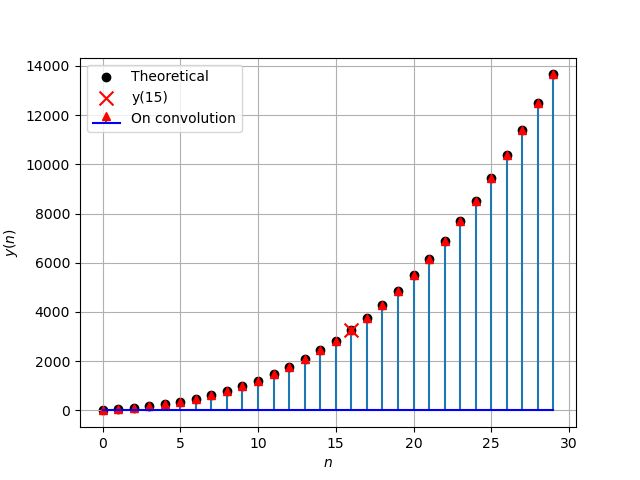
\includegraphics[width=\columnwidth]{ncert-maths/11/9/4/5/figs/plot.png}

\begin{center}
    \caption{Simulation v/s theoretical}
\end{center}
\end{figure}


\pagebreak

\item Write the five terms at n = 1, 2, 3, 4, 5 of the sequence and obtain the Z-transform of the series
\begin{align}
    x \brak{n} &=  -1, & n = 0 \\
    &=   \frac{x \brak{n-1}}{n}, & n > 0\\
    &=   0, & n < 0 
\end{align}

\solution

 \iffalse
\let\negmedspace\undefined
\let\negthickspace\undefined
\documentclass[journal,12pt,twocolumn]{IEEEtran}
\usepackage{amssymb}
\usepackage{cite}
\usepackage{amsmath,amssymb,amsfonts,amsthm}
\usepackage{algorithmic}
\usepackage{graphicx}
\usepackage{textcomp}
\usepackage{xcolor}
\usepackage{txfonts}
\usepackage{listings}
\usepackage{enumitem}
\usepackage{mathtools}
\usepackage{gensymb}
\usepackage{comment}
\usepackage[breaklinks=true]{hyperref}
\usepackage{tkz-euclide} 
\usepackage{listings}
\usepackage{gvv}                                        
\def\inputGnumericTable{}                                 
\usepackage[latin1]{inputenc}                                
\usepackage{color}                                            
\usepackage{array}                                            
\usepackage{longtable}                                       
\usepackage{calc}                                             
\usepackage{multirow}                                         
\usepackage{hhline}                                           
\usepackage{ifthen}                                           
\usepackage{lscape}
\usepackage{pgfplots}
\newtheorem{theorem}{Theorem}[section]
\newtheorem{problem}{Problem}
\newtheorem{proposition}{Proposition}[section]
\newtheorem{lemma}{Lemma}[section]
\newtheorem{corollary}[theorem]{Corollary}
\newtheorem{example}{Example}[section]
\newtheorem{definition}[problem]{Definition}
\newcommand{\BEQA}{\begin{eqnarray}}
\newcommand{\EEQA}{\end{eqnarray}}
\newcommand{\define}{\stackrel{\triangle}{=}}
\theoremstyle{remark}
\newtheorem{rem}{Remark}
\begin{document}

\bibliographystyle{IEEEtran}
\vspace{3cm}

\title{NCERT Discrete-11.9.4-5}
\author{EE22BTECH11004 - Allu Lohith}

\maketitle
\newpage
\bigskip


 Find the sum of n terms of this sequence:$$5^2+6^2+7^2...+20^2$$  
\solution
\fi
\begin{table}[h!]
\centering
\renewcommand{\arraystretch}{2}
\begin{tabular}{|c|p{4cm}|c|}
\hline 
\setlength{\tabcolsep}{1pt}
\textbf{Parameter}  &\textbf{Description} &\textbf{Formulae/Value} \\
\hline
n & Iteration number starting from zero till 15 & - \\
\hline
$x\brak n$ & General term of the sequence from $n=0$ to $n=15$ &$\brak{n+5}^2$  u\brak n\\
\hline
$x\brak 0$ & First term of the sequence & 5 \\
\hline
\end{tabular}

\vspace{0.5cm}
\caption{\normalsize Parameters}
\end{table}
The standard $z$ transforms,
\begin{align}
    u \brak n &\stackrel{z}{\longleftrightarrow} \frac{1}{1-z^{-1}}, \abs z >1\\
   n u\brak n &\stackrel{z}{\longleftrightarrow} \frac{z^{-1}}{\brak{1-z^{-1}}^2}, \abs z >1\\
   n^2 u\brak n &\stackrel{z}{\longleftrightarrow} \frac{z^{-1}\brak{1+z^{-1}}}{\brak{1-z^{-1}}^3}, \abs z >1
\end{align}
As 
\begin{align}
    x\brak n = \brak{n^2+10n+25}u\brak n
\end{align}
The $z$ transform of general term can be written as , 
\begin{align}
    X\brak z &= \frac{z^{-1}\brak{1+z^{-1}}}{\brak{1-z^{-1}}^3}+10\frac{z^{-1}}{\brak{1-z^{-1}}^2}+\frac{25}{1-z^{-1}} \\
    X\brak z &=  \frac{16z^{-2}-39z^{-1}+25}{\brak{1-z^{-1}}^3}; \abs{z}>1
\end{align}
On convolution for finding the sum
\begin{align}
    y\brak n= x\brak n \ast u\brak n
\end{align}
On z transform,
\begin{align}
    Y\brak z &= X \brak z \cdot U \brak z\\
    &= \brak{\frac{16z^{-2}-39z^{-1}+25}{\brak{1-z^{-1}})^3}} \cdot \frac{1}{1-z^{-1}}\\
    \implies 
    Y \brak z & = \frac{16z^{-2}-39z^{-1}+25}{\brak{1-z^{-1}}^4}; \quad \abs z >1
\end{align}
Using the contour integration to find the inverse $z$ transform,
\begin{align}
    y(n)&=\oint_c Y(z)\cdot z^{n-1}dz\\
    y(21)&=\oint_c \brak{\frac{16z^{-2}-39z^{-1}+25}{\brak{1-z^{-1}}^4}} z^{14}dz
\end{align}
As there are four poles from observation, so $m=4$
\begin{align}
    y\brak{21} &= \frac{1}{(m-1)!} \lim_{z \to a} \frac{d^{m-1}}{dz^{m-1}}\brak{(z-a)^mf(z)}\\
    &= \frac{1}{3!} \lim_{z \to 1} \frac{d^{3}}{dz^{3}}\brak{(z-1)^4 \frac{\brak{16z^{-2}-39z^{-1}+25}}{(1-z^{-1})^4} z^{14}}\\
    &= \frac{1}{6} \lim_{z \to 1} \frac{d^{3}}{dz^{3}}\brak{\brak{16z^{-2}-39z^{-1}+25}z^{18}}\\
    &= \frac{1}{6} \lim_{z \to 1} \frac{d^{3}}{dz^{3}}\brak{16z^{16}-39z^{17}+25z^{18}}\\
    &= \frac{1}{6}  \brak{16 \times 18 \times 17 \times 16+14 \times 17 \times 16 \times 15 }\\
    \implies y\brak{21}&=2840 
\end{align}
Hence the sum of the terms of the sequence is 2840.

\begin{figure}[h]
    \centering  

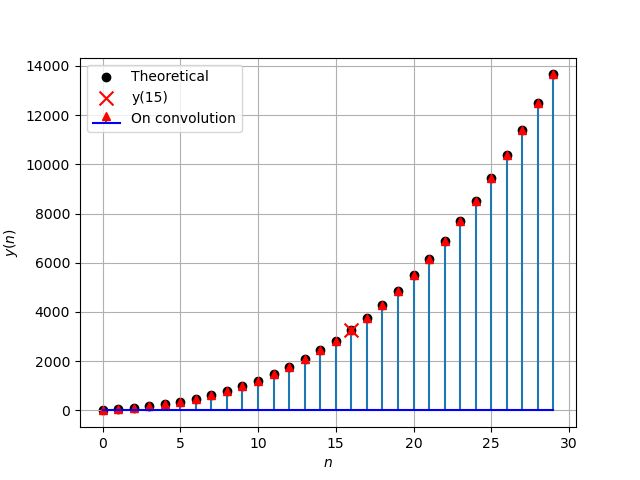
\includegraphics[width=\columnwidth]{ncert-maths/11/9/4/5/figs/plot.png}

\begin{center}
    \caption{Simulation v/s theoretical}
\end{center}
\end{figure}


\pagebreak


\item Subba Rao started work in 1995 at an annual salary of Rs. 5000 and received an increment of Rs. 200 each year. In which year did his income reach Rs. 7000?

\solution

 \iffalse
\let\negmedspace\undefined
\let\negthickspace\undefined
\documentclass[journal,12pt,twocolumn]{IEEEtran}
\usepackage{amssymb}
\usepackage{cite}
\usepackage{amsmath,amssymb,amsfonts,amsthm}
\usepackage{algorithmic}
\usepackage{graphicx}
\usepackage{textcomp}
\usepackage{xcolor}
\usepackage{txfonts}
\usepackage{listings}
\usepackage{enumitem}
\usepackage{mathtools}
\usepackage{gensymb}
\usepackage{comment}
\usepackage[breaklinks=true]{hyperref}
\usepackage{tkz-euclide} 
\usepackage{listings}
\usepackage{gvv}                                        
\def\inputGnumericTable{}                                 
\usepackage[latin1]{inputenc}                                
\usepackage{color}                                            
\usepackage{array}                                            
\usepackage{longtable}                                       
\usepackage{calc}                                             
\usepackage{multirow}                                         
\usepackage{hhline}                                           
\usepackage{ifthen}                                           
\usepackage{lscape}
\usepackage{pgfplots}
\newtheorem{theorem}{Theorem}[section]
\newtheorem{problem}{Problem}
\newtheorem{proposition}{Proposition}[section]
\newtheorem{lemma}{Lemma}[section]
\newtheorem{corollary}[theorem]{Corollary}
\newtheorem{example}{Example}[section]
\newtheorem{definition}[problem]{Definition}
\newcommand{\BEQA}{\begin{eqnarray}}
\newcommand{\EEQA}{\end{eqnarray}}
\newcommand{\define}{\stackrel{\triangle}{=}}
\theoremstyle{remark}
\newtheorem{rem}{Remark}
\begin{document}

\bibliographystyle{IEEEtran}
\vspace{3cm}

\title{NCERT Discrete-11.9.4-5}
\author{EE22BTECH11004 - Allu Lohith}

\maketitle
\newpage
\bigskip


 Find the sum of n terms of this sequence:$$5^2+6^2+7^2...+20^2$$  
\solution
\fi
\begin{table}[h!]
\centering
\renewcommand{\arraystretch}{2}
\begin{tabular}{|c|p{4cm}|c|}
\hline 
\setlength{\tabcolsep}{1pt}
\textbf{Parameter}  &\textbf{Description} &\textbf{Formulae/Value} \\
\hline
n & Iteration number starting from zero till 15 & - \\
\hline
$x\brak n$ & General term of the sequence from $n=0$ to $n=15$ &$\brak{n+5}^2$  u\brak n\\
\hline
$x\brak 0$ & First term of the sequence & 5 \\
\hline
\end{tabular}

\vspace{0.5cm}
\caption{\normalsize Parameters}
\end{table}
The standard $z$ transforms,
\begin{align}
    u \brak n &\stackrel{z}{\longleftrightarrow} \frac{1}{1-z^{-1}}, \abs z >1\\
   n u\brak n &\stackrel{z}{\longleftrightarrow} \frac{z^{-1}}{\brak{1-z^{-1}}^2}, \abs z >1\\
   n^2 u\brak n &\stackrel{z}{\longleftrightarrow} \frac{z^{-1}\brak{1+z^{-1}}}{\brak{1-z^{-1}}^3}, \abs z >1
\end{align}
As 
\begin{align}
    x\brak n = \brak{n^2+10n+25}u\brak n
\end{align}
The $z$ transform of general term can be written as , 
\begin{align}
    X\brak z &= \frac{z^{-1}\brak{1+z^{-1}}}{\brak{1-z^{-1}}^3}+10\frac{z^{-1}}{\brak{1-z^{-1}}^2}+\frac{25}{1-z^{-1}} \\
    X\brak z &=  \frac{16z^{-2}-39z^{-1}+25}{\brak{1-z^{-1}}^3}; \abs{z}>1
\end{align}
On convolution for finding the sum
\begin{align}
    y\brak n= x\brak n \ast u\brak n
\end{align}
On z transform,
\begin{align}
    Y\brak z &= X \brak z \cdot U \brak z\\
    &= \brak{\frac{16z^{-2}-39z^{-1}+25}{\brak{1-z^{-1}})^3}} \cdot \frac{1}{1-z^{-1}}\\
    \implies 
    Y \brak z & = \frac{16z^{-2}-39z^{-1}+25}{\brak{1-z^{-1}}^4}; \quad \abs z >1
\end{align}
Using the contour integration to find the inverse $z$ transform,
\begin{align}
    y(n)&=\oint_c Y(z)\cdot z^{n-1}dz\\
    y(21)&=\oint_c \brak{\frac{16z^{-2}-39z^{-1}+25}{\brak{1-z^{-1}}^4}} z^{14}dz
\end{align}
As there are four poles from observation, so $m=4$
\begin{align}
    y\brak{21} &= \frac{1}{(m-1)!} \lim_{z \to a} \frac{d^{m-1}}{dz^{m-1}}\brak{(z-a)^mf(z)}\\
    &= \frac{1}{3!} \lim_{z \to 1} \frac{d^{3}}{dz^{3}}\brak{(z-1)^4 \frac{\brak{16z^{-2}-39z^{-1}+25}}{(1-z^{-1})^4} z^{14}}\\
    &= \frac{1}{6} \lim_{z \to 1} \frac{d^{3}}{dz^{3}}\brak{\brak{16z^{-2}-39z^{-1}+25}z^{18}}\\
    &= \frac{1}{6} \lim_{z \to 1} \frac{d^{3}}{dz^{3}}\brak{16z^{16}-39z^{17}+25z^{18}}\\
    &= \frac{1}{6}  \brak{16 \times 18 \times 17 \times 16+14 \times 17 \times 16 \times 15 }\\
    \implies y\brak{21}&=2840 
\end{align}
Hence the sum of the terms of the sequence is 2840.

\begin{figure}[h]
    \centering  

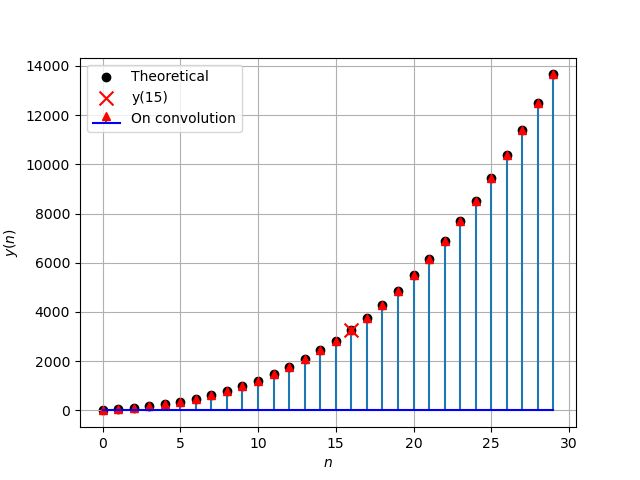
\includegraphics[width=\columnwidth]{ncert-maths/11/9/4/5/figs/plot.png}

\begin{center}
    \caption{Simulation v/s theoretical}
\end{center}
\end{figure}



\item Consider the sequence whose $n^\text{th}$ term is given by \(2^n\). Find the first 6 terms of this sequence.

\solution

\input{ncert-maths/11/9/1/3/2.tex}

\item If the sum of first 7 terms of an AP is 49 and that of 17 terms is 289, find the sum of first n terms.

\solution

 \iffalse
\let\negmedspace\undefined
\let\negthickspace\undefined
\documentclass[journal,12pt,twocolumn]{IEEEtran}
\usepackage{amssymb}
\usepackage{cite}
\usepackage{amsmath,amssymb,amsfonts,amsthm}
\usepackage{algorithmic}
\usepackage{graphicx}
\usepackage{textcomp}
\usepackage{xcolor}
\usepackage{txfonts}
\usepackage{listings}
\usepackage{enumitem}
\usepackage{mathtools}
\usepackage{gensymb}
\usepackage{comment}
\usepackage[breaklinks=true]{hyperref}
\usepackage{tkz-euclide} 
\usepackage{listings}
\usepackage{gvv}                                        
\def\inputGnumericTable{}                                 
\usepackage[latin1]{inputenc}                                
\usepackage{color}                                            
\usepackage{array}                                            
\usepackage{longtable}                                       
\usepackage{calc}                                             
\usepackage{multirow}                                         
\usepackage{hhline}                                           
\usepackage{ifthen}                                           
\usepackage{lscape}
\usepackage{pgfplots}
\newtheorem{theorem}{Theorem}[section]
\newtheorem{problem}{Problem}
\newtheorem{proposition}{Proposition}[section]
\newtheorem{lemma}{Lemma}[section]
\newtheorem{corollary}[theorem]{Corollary}
\newtheorem{example}{Example}[section]
\newtheorem{definition}[problem]{Definition}
\newcommand{\BEQA}{\begin{eqnarray}}
\newcommand{\EEQA}{\end{eqnarray}}
\newcommand{\define}{\stackrel{\triangle}{=}}
\theoremstyle{remark}
\newtheorem{rem}{Remark}
\begin{document}

\bibliographystyle{IEEEtran}
\vspace{3cm}

\title{NCERT Discrete-11.9.4-5}
\author{EE22BTECH11004 - Allu Lohith}

\maketitle
\newpage
\bigskip


 Find the sum of n terms of this sequence:$$5^2+6^2+7^2...+20^2$$  
\solution
\fi
\begin{table}[h!]
\centering
\renewcommand{\arraystretch}{2}
\begin{tabular}{|c|p{4cm}|c|}
\hline 
\setlength{\tabcolsep}{1pt}
\textbf{Parameter}  &\textbf{Description} &\textbf{Formulae/Value} \\
\hline
n & Iteration number starting from zero till 15 & - \\
\hline
$x\brak n$ & General term of the sequence from $n=0$ to $n=15$ &$\brak{n+5}^2$  u\brak n\\
\hline
$x\brak 0$ & First term of the sequence & 5 \\
\hline
\end{tabular}

\vspace{0.5cm}
\caption{\normalsize Parameters}
\end{table}
The standard $z$ transforms,
\begin{align}
    u \brak n &\stackrel{z}{\longleftrightarrow} \frac{1}{1-z^{-1}}, \abs z >1\\
   n u\brak n &\stackrel{z}{\longleftrightarrow} \frac{z^{-1}}{\brak{1-z^{-1}}^2}, \abs z >1\\
   n^2 u\brak n &\stackrel{z}{\longleftrightarrow} \frac{z^{-1}\brak{1+z^{-1}}}{\brak{1-z^{-1}}^3}, \abs z >1
\end{align}
As 
\begin{align}
    x\brak n = \brak{n^2+10n+25}u\brak n
\end{align}
The $z$ transform of general term can be written as , 
\begin{align}
    X\brak z &= \frac{z^{-1}\brak{1+z^{-1}}}{\brak{1-z^{-1}}^3}+10\frac{z^{-1}}{\brak{1-z^{-1}}^2}+\frac{25}{1-z^{-1}} \\
    X\brak z &=  \frac{16z^{-2}-39z^{-1}+25}{\brak{1-z^{-1}}^3}; \abs{z}>1
\end{align}
On convolution for finding the sum
\begin{align}
    y\brak n= x\brak n \ast u\brak n
\end{align}
On z transform,
\begin{align}
    Y\brak z &= X \brak z \cdot U \brak z\\
    &= \brak{\frac{16z^{-2}-39z^{-1}+25}{\brak{1-z^{-1}})^3}} \cdot \frac{1}{1-z^{-1}}\\
    \implies 
    Y \brak z & = \frac{16z^{-2}-39z^{-1}+25}{\brak{1-z^{-1}}^4}; \quad \abs z >1
\end{align}
Using the contour integration to find the inverse $z$ transform,
\begin{align}
    y(n)&=\oint_c Y(z)\cdot z^{n-1}dz\\
    y(21)&=\oint_c \brak{\frac{16z^{-2}-39z^{-1}+25}{\brak{1-z^{-1}}^4}} z^{14}dz
\end{align}
As there are four poles from observation, so $m=4$
\begin{align}
    y\brak{21} &= \frac{1}{(m-1)!} \lim_{z \to a} \frac{d^{m-1}}{dz^{m-1}}\brak{(z-a)^mf(z)}\\
    &= \frac{1}{3!} \lim_{z \to 1} \frac{d^{3}}{dz^{3}}\brak{(z-1)^4 \frac{\brak{16z^{-2}-39z^{-1}+25}}{(1-z^{-1})^4} z^{14}}\\
    &= \frac{1}{6} \lim_{z \to 1} \frac{d^{3}}{dz^{3}}\brak{\brak{16z^{-2}-39z^{-1}+25}z^{18}}\\
    &= \frac{1}{6} \lim_{z \to 1} \frac{d^{3}}{dz^{3}}\brak{16z^{16}-39z^{17}+25z^{18}}\\
    &= \frac{1}{6}  \brak{16 \times 18 \times 17 \times 16+14 \times 17 \times 16 \times 15 }\\
    \implies y\brak{21}&=2840 
\end{align}
Hence the sum of the terms of the sequence is 2840.

\begin{figure}[h]
    \centering  

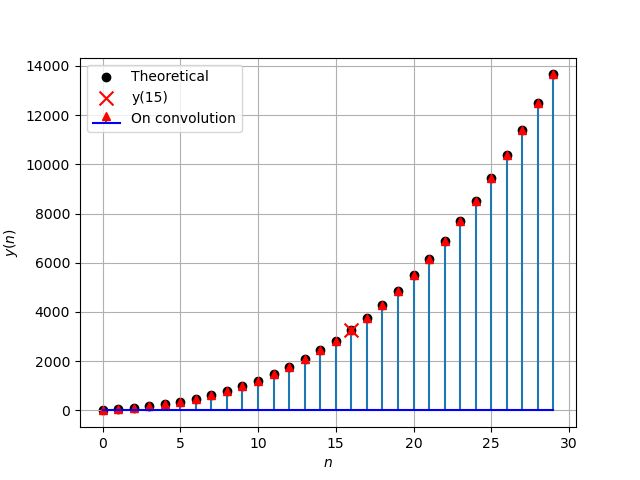
\includegraphics[width=\columnwidth]{ncert-maths/11/9/4/5/figs/plot.png}

\begin{center}
    \caption{Simulation v/s theoretical}
\end{center}
\end{figure}


\pagebreak

\item Write the first five terms of the sequence and obtain the corresponding series:\\
$a_1=a_2=2,$ $a_n=a_{n-1} -1,$ $n>2$\\
\solution
 \iffalse
\let\negmedspace\undefined
\let\negthickspace\undefined
\documentclass[journal,12pt,twocolumn]{IEEEtran}
\usepackage{amssymb}
\usepackage{cite}
\usepackage{amsmath,amssymb,amsfonts,amsthm}
\usepackage{algorithmic}
\usepackage{graphicx}
\usepackage{textcomp}
\usepackage{xcolor}
\usepackage{txfonts}
\usepackage{listings}
\usepackage{enumitem}
\usepackage{mathtools}
\usepackage{gensymb}
\usepackage{comment}
\usepackage[breaklinks=true]{hyperref}
\usepackage{tkz-euclide} 
\usepackage{listings}
\usepackage{gvv}                                        
\def\inputGnumericTable{}                                 
\usepackage[latin1]{inputenc}                                
\usepackage{color}                                            
\usepackage{array}                                            
\usepackage{longtable}                                       
\usepackage{calc}                                             
\usepackage{multirow}                                         
\usepackage{hhline}                                           
\usepackage{ifthen}                                           
\usepackage{lscape}
\usepackage{pgfplots}
\newtheorem{theorem}{Theorem}[section]
\newtheorem{problem}{Problem}
\newtheorem{proposition}{Proposition}[section]
\newtheorem{lemma}{Lemma}[section]
\newtheorem{corollary}[theorem]{Corollary}
\newtheorem{example}{Example}[section]
\newtheorem{definition}[problem]{Definition}
\newcommand{\BEQA}{\begin{eqnarray}}
\newcommand{\EEQA}{\end{eqnarray}}
\newcommand{\define}{\stackrel{\triangle}{=}}
\theoremstyle{remark}
\newtheorem{rem}{Remark}
\begin{document}

\bibliographystyle{IEEEtran}
\vspace{3cm}

\title{NCERT Discrete-11.9.4-5}
\author{EE22BTECH11004 - Allu Lohith}

\maketitle
\newpage
\bigskip


 Find the sum of n terms of this sequence:$$5^2+6^2+7^2...+20^2$$  
\solution
\fi
\begin{table}[h!]
\centering
\renewcommand{\arraystretch}{2}
\begin{tabular}{|c|p{4cm}|c|}
\hline 
\setlength{\tabcolsep}{1pt}
\textbf{Parameter}  &\textbf{Description} &\textbf{Formulae/Value} \\
\hline
n & Iteration number starting from zero till 15 & - \\
\hline
$x\brak n$ & General term of the sequence from $n=0$ to $n=15$ &$\brak{n+5}^2$  u\brak n\\
\hline
$x\brak 0$ & First term of the sequence & 5 \\
\hline
\end{tabular}

\vspace{0.5cm}
\caption{\normalsize Parameters}
\end{table}
The standard $z$ transforms,
\begin{align}
    u \brak n &\stackrel{z}{\longleftrightarrow} \frac{1}{1-z^{-1}}, \abs z >1\\
   n u\brak n &\stackrel{z}{\longleftrightarrow} \frac{z^{-1}}{\brak{1-z^{-1}}^2}, \abs z >1\\
   n^2 u\brak n &\stackrel{z}{\longleftrightarrow} \frac{z^{-1}\brak{1+z^{-1}}}{\brak{1-z^{-1}}^3}, \abs z >1
\end{align}
As 
\begin{align}
    x\brak n = \brak{n^2+10n+25}u\brak n
\end{align}
The $z$ transform of general term can be written as , 
\begin{align}
    X\brak z &= \frac{z^{-1}\brak{1+z^{-1}}}{\brak{1-z^{-1}}^3}+10\frac{z^{-1}}{\brak{1-z^{-1}}^2}+\frac{25}{1-z^{-1}} \\
    X\brak z &=  \frac{16z^{-2}-39z^{-1}+25}{\brak{1-z^{-1}}^3}; \abs{z}>1
\end{align}
On convolution for finding the sum
\begin{align}
    y\brak n= x\brak n \ast u\brak n
\end{align}
On z transform,
\begin{align}
    Y\brak z &= X \brak z \cdot U \brak z\\
    &= \brak{\frac{16z^{-2}-39z^{-1}+25}{\brak{1-z^{-1}})^3}} \cdot \frac{1}{1-z^{-1}}\\
    \implies 
    Y \brak z & = \frac{16z^{-2}-39z^{-1}+25}{\brak{1-z^{-1}}^4}; \quad \abs z >1
\end{align}
Using the contour integration to find the inverse $z$ transform,
\begin{align}
    y(n)&=\oint_c Y(z)\cdot z^{n-1}dz\\
    y(21)&=\oint_c \brak{\frac{16z^{-2}-39z^{-1}+25}{\brak{1-z^{-1}}^4}} z^{14}dz
\end{align}
As there are four poles from observation, so $m=4$
\begin{align}
    y\brak{21} &= \frac{1}{(m-1)!} \lim_{z \to a} \frac{d^{m-1}}{dz^{m-1}}\brak{(z-a)^mf(z)}\\
    &= \frac{1}{3!} \lim_{z \to 1} \frac{d^{3}}{dz^{3}}\brak{(z-1)^4 \frac{\brak{16z^{-2}-39z^{-1}+25}}{(1-z^{-1})^4} z^{14}}\\
    &= \frac{1}{6} \lim_{z \to 1} \frac{d^{3}}{dz^{3}}\brak{\brak{16z^{-2}-39z^{-1}+25}z^{18}}\\
    &= \frac{1}{6} \lim_{z \to 1} \frac{d^{3}}{dz^{3}}\brak{16z^{16}-39z^{17}+25z^{18}}\\
    &= \frac{1}{6}  \brak{16 \times 18 \times 17 \times 16+14 \times 17 \times 16 \times 15 }\\
    \implies y\brak{21}&=2840 
\end{align}
Hence the sum of the terms of the sequence is 2840.

\begin{figure}[h]
    \centering  

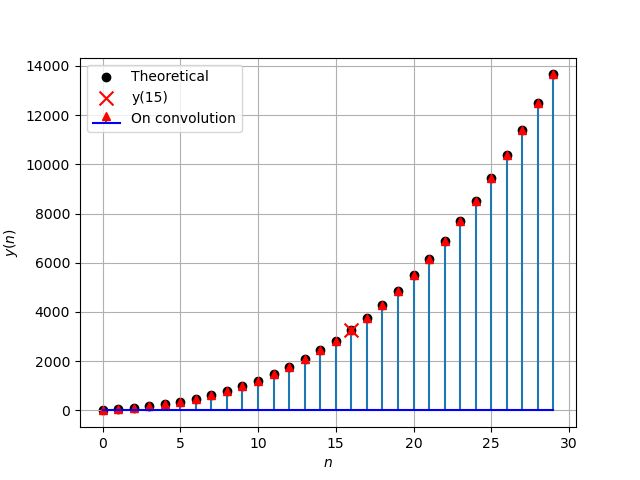
\includegraphics[width=\columnwidth]{ncert-maths/11/9/4/5/figs/plot.png}

\begin{center}
    \caption{Simulation v/s theoretical}
\end{center}
\end{figure}


\pagebreak
\item Insert two numbers between 3 and 81 so that the resulting sequence is G.P.\\

\solution
\input{ncert-maths/11/9/3/26/asnmt1.tex}
\pagebreak

\item  What will Rs 500 amounts to in 10 years after its deposit in a bank which pays annual interest rate of 10$\%$ compounded annually?

\solution
     \iffalse
\let\negmedspace\undefined
\let\negthickspace\undefined
\documentclass[journal,12pt,twocolumn]{IEEEtran}
\usepackage{amssymb}
\usepackage{cite}
\usepackage{amsmath,amssymb,amsfonts,amsthm}
\usepackage{algorithmic}
\usepackage{graphicx}
\usepackage{textcomp}
\usepackage{xcolor}
\usepackage{txfonts}
\usepackage{listings}
\usepackage{enumitem}
\usepackage{mathtools}
\usepackage{gensymb}
\usepackage{comment}
\usepackage[breaklinks=true]{hyperref}
\usepackage{tkz-euclide} 
\usepackage{listings}
\usepackage{gvv}                                        
\def\inputGnumericTable{}                                 
\usepackage[latin1]{inputenc}                                
\usepackage{color}                                            
\usepackage{array}                                            
\usepackage{longtable}                                       
\usepackage{calc}                                             
\usepackage{multirow}                                         
\usepackage{hhline}                                           
\usepackage{ifthen}                                           
\usepackage{lscape}
\usepackage{pgfplots}
\newtheorem{theorem}{Theorem}[section]
\newtheorem{problem}{Problem}
\newtheorem{proposition}{Proposition}[section]
\newtheorem{lemma}{Lemma}[section]
\newtheorem{corollary}[theorem]{Corollary}
\newtheorem{example}{Example}[section]
\newtheorem{definition}[problem]{Definition}
\newcommand{\BEQA}{\begin{eqnarray}}
\newcommand{\EEQA}{\end{eqnarray}}
\newcommand{\define}{\stackrel{\triangle}{=}}
\theoremstyle{remark}
\newtheorem{rem}{Remark}
\begin{document}

\bibliographystyle{IEEEtran}
\vspace{3cm}

\title{NCERT Discrete-11.9.4-5}
\author{EE22BTECH11004 - Allu Lohith}

\maketitle
\newpage
\bigskip


 Find the sum of n terms of this sequence:$$5^2+6^2+7^2...+20^2$$  
\solution
\fi
\begin{table}[h!]
\centering
\renewcommand{\arraystretch}{2}
\begin{tabular}{|c|p{4cm}|c|}
\hline 
\setlength{\tabcolsep}{1pt}
\textbf{Parameter}  &\textbf{Description} &\textbf{Formulae/Value} \\
\hline
n & Iteration number starting from zero till 15 & - \\
\hline
$x\brak n$ & General term of the sequence from $n=0$ to $n=15$ &$\brak{n+5}^2$  u\brak n\\
\hline
$x\brak 0$ & First term of the sequence & 5 \\
\hline
\end{tabular}

\vspace{0.5cm}
\caption{\normalsize Parameters}
\end{table}
The standard $z$ transforms,
\begin{align}
    u \brak n &\stackrel{z}{\longleftrightarrow} \frac{1}{1-z^{-1}}, \abs z >1\\
   n u\brak n &\stackrel{z}{\longleftrightarrow} \frac{z^{-1}}{\brak{1-z^{-1}}^2}, \abs z >1\\
   n^2 u\brak n &\stackrel{z}{\longleftrightarrow} \frac{z^{-1}\brak{1+z^{-1}}}{\brak{1-z^{-1}}^3}, \abs z >1
\end{align}
As 
\begin{align}
    x\brak n = \brak{n^2+10n+25}u\brak n
\end{align}
The $z$ transform of general term can be written as , 
\begin{align}
    X\brak z &= \frac{z^{-1}\brak{1+z^{-1}}}{\brak{1-z^{-1}}^3}+10\frac{z^{-1}}{\brak{1-z^{-1}}^2}+\frac{25}{1-z^{-1}} \\
    X\brak z &=  \frac{16z^{-2}-39z^{-1}+25}{\brak{1-z^{-1}}^3}; \abs{z}>1
\end{align}
On convolution for finding the sum
\begin{align}
    y\brak n= x\brak n \ast u\brak n
\end{align}
On z transform,
\begin{align}
    Y\brak z &= X \brak z \cdot U \brak z\\
    &= \brak{\frac{16z^{-2}-39z^{-1}+25}{\brak{1-z^{-1}})^3}} \cdot \frac{1}{1-z^{-1}}\\
    \implies 
    Y \brak z & = \frac{16z^{-2}-39z^{-1}+25}{\brak{1-z^{-1}}^4}; \quad \abs z >1
\end{align}
Using the contour integration to find the inverse $z$ transform,
\begin{align}
    y(n)&=\oint_c Y(z)\cdot z^{n-1}dz\\
    y(21)&=\oint_c \brak{\frac{16z^{-2}-39z^{-1}+25}{\brak{1-z^{-1}}^4}} z^{14}dz
\end{align}
As there are four poles from observation, so $m=4$
\begin{align}
    y\brak{21} &= \frac{1}{(m-1)!} \lim_{z \to a} \frac{d^{m-1}}{dz^{m-1}}\brak{(z-a)^mf(z)}\\
    &= \frac{1}{3!} \lim_{z \to 1} \frac{d^{3}}{dz^{3}}\brak{(z-1)^4 \frac{\brak{16z^{-2}-39z^{-1}+25}}{(1-z^{-1})^4} z^{14}}\\
    &= \frac{1}{6} \lim_{z \to 1} \frac{d^{3}}{dz^{3}}\brak{\brak{16z^{-2}-39z^{-1}+25}z^{18}}\\
    &= \frac{1}{6} \lim_{z \to 1} \frac{d^{3}}{dz^{3}}\brak{16z^{16}-39z^{17}+25z^{18}}\\
    &= \frac{1}{6}  \brak{16 \times 18 \times 17 \times 16+14 \times 17 \times 16 \times 15 }\\
    \implies y\brak{21}&=2840 
\end{align}
Hence the sum of the terms of the sequence is 2840.

\begin{figure}[h]
    \centering  

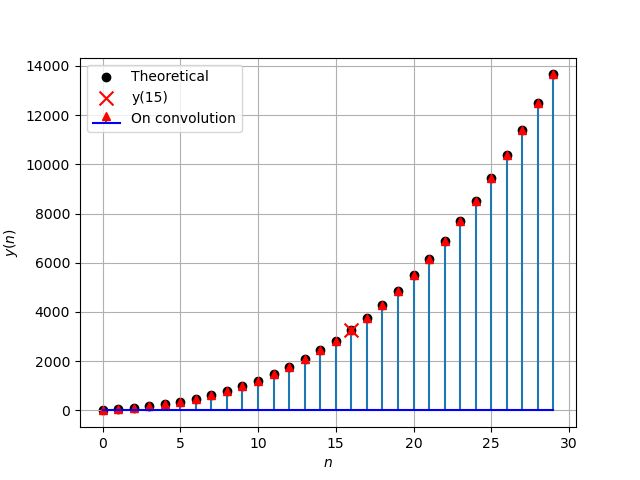
\includegraphics[width=\columnwidth]{ncert-maths/11/9/4/5/figs/plot.png}

\begin{center}
    \caption{Simulation v/s theoretical}
\end{center}
\end{figure}


\pagebreak

\item Find the $20^{th}$ term from the last term of the AP: $3,8,13.....253$.

\solution
 \iffalse
\let\negmedspace\undefined
\let\negthickspace\undefined
\documentclass[journal,12pt,twocolumn]{IEEEtran}
\usepackage{amssymb}
\usepackage{cite}
\usepackage{amsmath,amssymb,amsfonts,amsthm}
\usepackage{algorithmic}
\usepackage{graphicx}
\usepackage{textcomp}
\usepackage{xcolor}
\usepackage{txfonts}
\usepackage{listings}
\usepackage{enumitem}
\usepackage{mathtools}
\usepackage{gensymb}
\usepackage{comment}
\usepackage[breaklinks=true]{hyperref}
\usepackage{tkz-euclide} 
\usepackage{listings}
\usepackage{gvv}                                        
\def\inputGnumericTable{}                                 
\usepackage[latin1]{inputenc}                                
\usepackage{color}                                            
\usepackage{array}                                            
\usepackage{longtable}                                       
\usepackage{calc}                                             
\usepackage{multirow}                                         
\usepackage{hhline}                                           
\usepackage{ifthen}                                           
\usepackage{lscape}
\usepackage{pgfplots}
\newtheorem{theorem}{Theorem}[section]
\newtheorem{problem}{Problem}
\newtheorem{proposition}{Proposition}[section]
\newtheorem{lemma}{Lemma}[section]
\newtheorem{corollary}[theorem]{Corollary}
\newtheorem{example}{Example}[section]
\newtheorem{definition}[problem]{Definition}
\newcommand{\BEQA}{\begin{eqnarray}}
\newcommand{\EEQA}{\end{eqnarray}}
\newcommand{\define}{\stackrel{\triangle}{=}}
\theoremstyle{remark}
\newtheorem{rem}{Remark}
\begin{document}

\bibliographystyle{IEEEtran}
\vspace{3cm}

\title{NCERT Discrete-11.9.4-5}
\author{EE22BTECH11004 - Allu Lohith}

\maketitle
\newpage
\bigskip


 Find the sum of n terms of this sequence:$$5^2+6^2+7^2...+20^2$$  
\solution
\fi
\begin{table}[h!]
\centering
\renewcommand{\arraystretch}{2}
\begin{tabular}{|c|p{4cm}|c|}
\hline 
\setlength{\tabcolsep}{1pt}
\textbf{Parameter}  &\textbf{Description} &\textbf{Formulae/Value} \\
\hline
n & Iteration number starting from zero till 15 & - \\
\hline
$x\brak n$ & General term of the sequence from $n=0$ to $n=15$ &$\brak{n+5}^2$  u\brak n\\
\hline
$x\brak 0$ & First term of the sequence & 5 \\
\hline
\end{tabular}

\vspace{0.5cm}
\caption{\normalsize Parameters}
\end{table}
The standard $z$ transforms,
\begin{align}
    u \brak n &\stackrel{z}{\longleftrightarrow} \frac{1}{1-z^{-1}}, \abs z >1\\
   n u\brak n &\stackrel{z}{\longleftrightarrow} \frac{z^{-1}}{\brak{1-z^{-1}}^2}, \abs z >1\\
   n^2 u\brak n &\stackrel{z}{\longleftrightarrow} \frac{z^{-1}\brak{1+z^{-1}}}{\brak{1-z^{-1}}^3}, \abs z >1
\end{align}
As 
\begin{align}
    x\brak n = \brak{n^2+10n+25}u\brak n
\end{align}
The $z$ transform of general term can be written as , 
\begin{align}
    X\brak z &= \frac{z^{-1}\brak{1+z^{-1}}}{\brak{1-z^{-1}}^3}+10\frac{z^{-1}}{\brak{1-z^{-1}}^2}+\frac{25}{1-z^{-1}} \\
    X\brak z &=  \frac{16z^{-2}-39z^{-1}+25}{\brak{1-z^{-1}}^3}; \abs{z}>1
\end{align}
On convolution for finding the sum
\begin{align}
    y\brak n= x\brak n \ast u\brak n
\end{align}
On z transform,
\begin{align}
    Y\brak z &= X \brak z \cdot U \brak z\\
    &= \brak{\frac{16z^{-2}-39z^{-1}+25}{\brak{1-z^{-1}})^3}} \cdot \frac{1}{1-z^{-1}}\\
    \implies 
    Y \brak z & = \frac{16z^{-2}-39z^{-1}+25}{\brak{1-z^{-1}}^4}; \quad \abs z >1
\end{align}
Using the contour integration to find the inverse $z$ transform,
\begin{align}
    y(n)&=\oint_c Y(z)\cdot z^{n-1}dz\\
    y(21)&=\oint_c \brak{\frac{16z^{-2}-39z^{-1}+25}{\brak{1-z^{-1}}^4}} z^{14}dz
\end{align}
As there are four poles from observation, so $m=4$
\begin{align}
    y\brak{21} &= \frac{1}{(m-1)!} \lim_{z \to a} \frac{d^{m-1}}{dz^{m-1}}\brak{(z-a)^mf(z)}\\
    &= \frac{1}{3!} \lim_{z \to 1} \frac{d^{3}}{dz^{3}}\brak{(z-1)^4 \frac{\brak{16z^{-2}-39z^{-1}+25}}{(1-z^{-1})^4} z^{14}}\\
    &= \frac{1}{6} \lim_{z \to 1} \frac{d^{3}}{dz^{3}}\brak{\brak{16z^{-2}-39z^{-1}+25}z^{18}}\\
    &= \frac{1}{6} \lim_{z \to 1} \frac{d^{3}}{dz^{3}}\brak{16z^{16}-39z^{17}+25z^{18}}\\
    &= \frac{1}{6}  \brak{16 \times 18 \times 17 \times 16+14 \times 17 \times 16 \times 15 }\\
    \implies y\brak{21}&=2840 
\end{align}
Hence the sum of the terms of the sequence is 2840.

\begin{figure}[h]
    \centering  

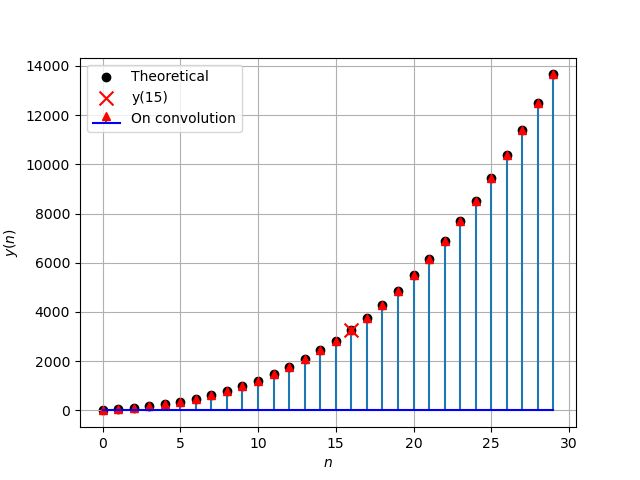
\includegraphics[width=\columnwidth]{ncert-maths/11/9/4/5/figs/plot.png}

\begin{center}
    \caption{Simulation v/s theoretical}
\end{center}
\end{figure}



\pagebreak
\item Find the sum to $n$ terms of series , whose $n^{th}$ term is : $n(n+1)(n+4)$.

\solution
\input{ncert-maths/11/9/4/8/math.11.9.4.8.tex}
\pagebreak

\item Find the indicated terms in the sequence whose nth terms is $a(n)$ = $4n-3$. Find $a(17)$ and $a(24)$.
    
\solution 
\input{ncert-maths/11/9/1/7/7.tex}
\pagebreak

\item The difference between any two cosecutive interior angles of a polygon is $5^\circ$.If the smallest angle is $120^\circ$,find the number of sides of polygon. \\
\solution
\input{ncert-maths/11/9/2/18/ass_1.tex}
\pagebreak
\item The $5$th,$8$th and $11$th terms of a GP are p,q and s respectively .show that $q^2=ps$ \\
\solution
\input{ncert-maths/11/9/3/3/assign1.tex}
\pagebreak
\item The sum of the first four terms of an A.P. is 56. The sum of the last four terms is
 112. If its first term is 11, then find the number of terms.\\
\solution
\input{ncert-maths/11/9/5/12/Assignment2.tex}
\pagebreak
\item Find the sum to $n$ terms of the series whose $n^{th}$ term is given by $(2n-1)^2$ ? 
\solution
\input{ncert-maths/11/9/4/10/2.1.tex}
\pagebreak
\item If the $4^{th}$, $10^{th}$ and $16^{th}$ terms of a G.P. are $x$, $y$, and $z$, respectively. Prove that $x,\; y,\; z$ are in G.P. \\
\solution
\input{ncert-maths/11/9/3/17/A_1.tex}
\pagebreak
\item Show that the ratio of the sum of the first \(n\) terms of a geometric progression (G.P.) to the sum of terms from \((n+1)\)th to \((2n)\)th term is \(\frac{1}{r^n}\).
\solution
\iffalse
\let\negmedspace\undefined
\let\negthickspace\undefined
\documentclass[journal,12pt,twocolumn]{IEEEtran}
\usepackage{cite}
\usepackage{amsmath,amssymb,amsfonts,amsthm}

\usepackage{graphicx}
\usepackage{textcomp}
\usepackage{xcolor}
\usepackage{txfonts}
\usepackage{listings}
\usepackage{enumitem}
\usepackage{mathtools}
\usepackage{gensymb}
\usepackage[breaklinks=true]{hyperref}
\usepackage{tkz-euclide} % loads  TikZ and tkz-base
\usepackage{listings}
\usepackage{gvv}
\usepackage{booktabs}

%
%\usepackage{setspace}
%\usepackage{gensymb}
%\doublespacing
%\singlespacing

%\usepackage{graphicx}
%\usepackage{amssymb}
%\usepackage{relsize}
%\usepackage[cmex10]{amsmath}
%\usepackage{amsthm}
%\interdisplaylinepenalty=2500
%\savesymbol{iint}
%\usepackage{txfonts}
%\restoresymbol{TXF}{iint}
%\usepackage{wasysym}
%\usepackage{amsthm}
%\usepackage{iithtlc}
%\usepackage{mathrsfs}
%\usepackage{txfonts}
%\usepackage{stfloats}
%\usepackage{bm}
%\usepackage{cite}
%\usepackage{cases}
%\usepackage{subfig}
%\usepackage{xtab}
%\usepackage{longtable}
%\usepackage{multirow}

%\usepackage{algpseudocode}
%\usepackage{enumitem}
%\usepackage{mathtools}
%\usepackage{tikz}
%\usepackage{circuitikz}
%\usepackage{verbatim}
%\usepackage{tfrupee}
%\usepackage{stmaryrd}
%\usetkzobj{all}
%    \usepackage{color}                                            %%
%    \usepackage{array}                                            %%
%    \usepackage{longtable}                                        %%
%    \usepackage{calc}                                             %%
%    \usepackage{multirow}                                         %%
%    \usepackage{hhline}                                           %%
%    \usepackage{ifthen}                                           %%
  %optionally (for landscape tables embedded in another document): %%
%    \usepackage{lscape}     
%\usepackage{multicol}
%\usepackage{chngcntr}
%\usepackage{enumerate}

%\usepackage{wasysym}
%\documentclass[conference]{IEEEtran}
%\IEEEoverridecommandlockouts
% The preceding line is only needed to identify funding in the first footnote. If that is unneeded, please comment it out.

\newtheorem{theorem}{Theorem}[section]
\newtheorem{problem}{Problem}
\newtheorem{proposition}{Proposition}[section]
\newtheorem{lemma}{Lemma}[section]
\newtheorem{corollary}[theorem]{Corollary}
\newtheorem{example}{Example}[section]
\newtheorem{definition}[problem]{Definition}
%\newtheorem{thm}{Theorem}[section] 
%\newtheorem{defn}[thm]{Definition}
%\newtheorem{algorithm}{Algorithm}[section]
%\newtheorem{cor}{Corollary}
\newcommand{\BEQA}{\begin{eqnarray}}
\newcommand{\EEQA}{\end{eqnarray}}
\newcommand{\define}{\stackrel{\triangle}{=}}
\theoremstyle{remark}
\newtheorem{rem}{Remark}

%\bibliographystyle{ieeetr}
\begin{document}
%

\bibliographystyle{IEEEtran}


\vspace{3cm}

\title{
%	\logo{
Discrete Assignment 

\large{EE:1205 Signals and Systems}

Indian Institute of Technology, Hyderabad
%	}
}
\author{Abhey Garg

EE23BTECH11202
}	


% make the title area
\maketitle

\newpage

%\tableofcontents

\bigskip

\renewcommand{\thefigure}{\theenumi}
\renewcommand{\thetable}{\theenumi}
%\renewcommand{\theequation}{\theenumi}

\section{Question 11.9.3.24}
Show that the ratio of the sum of the first \(n\) terms of a geometric progression (G.P.) to the sum of terms from \((n+1)\)th to \((2n)\)th term is \(\frac{1}{r^n}\).
\section{Solution}
\fi
\begin{table}[htbp]
\centering
\caption{Input Parameters}
\begin{tabular}{|p{1cm}|p{2.5cm}|p{2cm}|}
\hline
\textbf{Variable} & \textbf{Description} & \textbf{Value} \\
\hline
$x(0)$ &  First term of G.P & \\
\hline
$r$ & Common ratio of G.P & \\
\hline
$x(n)$ & General Term & $x(0) \cdot r^n \cdot u(n)$ \\
\hline

\end{tabular}

\end{table}
\begin{equation}
x(n) = x(0) r^n u(n)
\end{equation}

where

\[
u(n) = 
\begin{cases} 
0 & \text{for } n < 0 \\
1 & \text{for } n \geq 0 
\end{cases}
\]
\begin{align}
y(n) &= \sum_{k=-\infty}^{n} x(k) \\
y(n) &= x(n)*u(n)
\end{align}
Taking z transform
\begin{align}
Y(z) = X(z)U(z)
\end{align}
\begin{align}
= \left(\frac{x(0)}{1 - rz^{-1}}\right) \left(\frac{1}{1 - z^{-1}}\right)  \quad |z| > |r| \cap |z| > 1
\end{align}
\begin{align}
= \frac{x(0)}{(1 - rz^{-1})(1 - z^{-1})} && \quad |z| > |r|
\end{align}
which can be expressed as
\begin{align}
Y(z) = \frac{x(0)}{r-1} \left(\frac{r}{1-rz^{-1}} - \frac{1}{1-z^{-1}}\right)
\end{align}
Using partial fractions, again the inverse of the above can be expressed as 
\begin{align}
y(n) = x(0)\left(\frac{r^{n}-1}{r-1}\right)u(n)
\end{align}
\begin{align}
y(2n) = x(0)\left(\frac{r^{2n-1}-1}{r-1}\right)u(2n)
\end{align}
Now we have to find $\frac{y(n)}{y(2n)-y(n)}$
\begin{align}
\frac{y(n)}{y(2n)-y(n)} = \frac{x(0)\left(\frac{r^{n}-1}{r-1}\right)u(n)}{x(0)\left(\frac{r^{2n}-1}{r-1}\right)u(2n)- x(0)\left(\frac{r^{n}-1}{r-1}\right)u(n)}
\end{align}
\begin{align}
 = \frac{\left(\frac{r^{n}-1}{r-1}\right)}{\left(\frac{r^{2n}-1}{r-1}\right)- \left(\frac{r^{n}-1}{r-1}\right)}
\end{align}
\begin{align}
= \frac{r^{n}-1}{(r^{2n}-1)- (r^{n}-1)}
\end{align}
\begin{align}
= \frac{r^{n}}{(r^{2n})- (r^{n})}
\end{align}
\begin{align}
= \frac{1}{r^{n}}
\end{align}
\begin{figure}[!ht]
\centering
\begin{center}
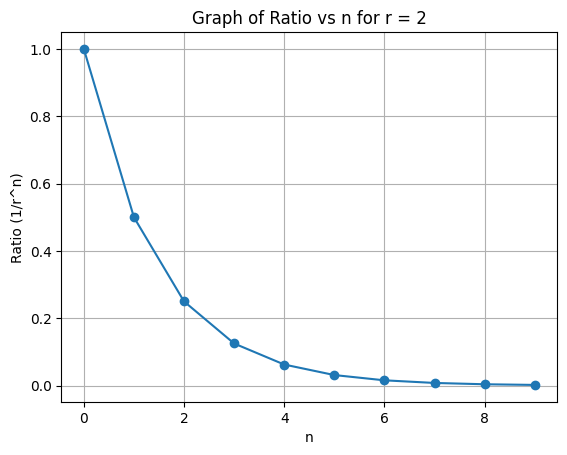
\includegraphics[width=\columnwidth]{ncert-maths/11/9/3/24/figs/figure1.png}
\caption{Plot of ratio vs $1/r^n$ for r = 2}
\end{center}
\end{figure}

%\end{document}

\pagebreak
\item A G.P consists of an even number of terms. If the sum of all terms is 5 times the sum of terms occupying odd places, then find its common ratio.\\
\solution
\input{ncert-maths/11/9/5/11/firstcorrection.tex}
\pagebreak
\item Find the sum to indicated number of terms in the geometric progression $x^3,x^5,x^7,...n$ terms (if $x\neq\pm1$).\\
\solution
\input{ncert-maths/11/9/3/10/11.9.3.Q10.tex}
\pagebreak
\item Determine the AP whose third term is 16 and the 7th term exceeds the 5th term by 12. \\
\solution
\input{ncert-maths/10/5/2/16/1.tex}
\pagebreak
\item Find the seventh term of the sequence where the nth term is given by $a_n= \frac {n^2}{2^{n}}$\\
\solution
\input{ncert-maths/11/9/1/8/a1.tex}
\pagebreak
\item Find sum to n terms of the following series:\\
$\frac{1}{1 \times 2} + \frac{1}{2 \times 3} + \frac{1}{3 \times 4} + \ldots$ \hfill(NCERT 11.9.4.4)\\
\solution
\input{ncert-maths/11/9/9/4/11.9.9.4.tex} 
\pagebreak
\item 1x2x3 + 2x3x4 + 3x4x5 +..... \\
\solution
\let\negmedspace\undefined
\let\negthickspace\undefined
\documentclass[journal,12pt,twocolumn]{IEEEtran}
\usepackage{cite}
\usepackage{amsmath,amssymb,amsfonts,amsthm}
\usepackage{algorithmic}
\usepackage{graphicx}
\usepackage{textcomp}
\usepackage{xcolor}
\usepackage{txfonts}
\usepackage{listings}
\usepackage{enumitem}
\usepackage{mathtools}
\usepackage{gensymb}
\usepackage[breaklinks=true]{hyperref}
\usepackage{tkz-euclide} % loads  TikZ and tkz-base
\usepackage{listings}
\usepackage{gvv}
%
%\usepackage{setspace}
%\usepackage{gensymb}
%\doublespacing
%\singlespacing

%\usepackage{graphicx}
%\usepackage{amssymb}
%\usepackage{relsize}
%\usepackage[cmex10]{amsmath}
%\usepackage{amsthm}
%\interdisplaylinepenalty=2500
%\savesymbol{iint}
%\usepackage{txfonts}
%\restoresymbol{TXF}{iint}
%\usepackage{wasysym}
%\usepackage{amsthm}
%\usepackage{iithtlc}
%\usepackage{mathrsfs}
%\usepackage{txfonts}
%\usepackage{stfloats}
%\usepackage{bm}
%\usepackage{cite}
%\usepackage{cases}
%\usepackage{subfig}
%\usepackage{xtab}
%\usepackage{longtable}
%\usepackage{multirow}
%\usepackage{algorithm}
%\usepackage{algpseudocode}
%\usepackage{enumitem}
%\usepackage{mathtools}
%\usepackage{tikz}
%\usepackage{circuitikz}
%\usepackage{verbatim}
%\usepackage{tfrupee}
%\usepackage{stmaryrd}
%\usetkzobj{all}
%    \usepackage{color}                                            %%
%    \usepackage{array}                                            %%
%    \usepackage{longtable}                                        %%
%    \usepackage{calc}                                             %%
%    \usepackage{multirow}                                         %%
%    \usepackage{hhline}                                           %%
%    \usepackage{ifthen}                                           %%
  %optionally (for landscape tables embedded in another document): %%
%    \usepackage{lscape}     
%\usepackage{multicol}
%\usepackage{chngcntr}
%\usepackage{enumerate}

%\usepackage{wasysym}
%\documentclass[conference]{IEEEtran}
%\IEEEoverridecommandlockouts
% The preceding line is only needed to identify funding in the first footnote. If that is unneeded, please comment it out.

\newtheorem{theorem}{Theorem}[section]
\newtheorem{problem}{Problem}
\newtheorem{proposition}{Proposition}[section]
\newtheorem{lemma}{Lemma}[section]
\newtheorem{corollary}[theorem]{Corollary}
\newtheorem{example}{Example}[section]
\newtheorem{definition}[problem]{Definition}
%\newtheorem{thm}{Theorem}[section] 
%\newtheorem{defn}[thm]{Definition}
%\newtheorem{algorithm}{Algorithm}[section]
%\newtheorem{cor}{Corollary}
\newcommand{\BEQA}{\begin{eqnarray}}
\newcommand{\EEQA}{\end{eqnarray}}
\newcommand{\define}{\stackrel{\triangle}{=}}
\theoremstyle{remark}
\newtheorem{rem}{Remark}

%\bibliographystyle{ieeetr}
\begin{document}
%

\bibliographystyle{IEEEtran}


\vspace{3cm}

\title{
%	\logo{
Assignment-3

\large{EE:1205 Signals and systems}

Indian Institute of Technology, Hyderabad
%	}
}
\author{Sai Preetam Umesh Sasankota

EE23BTECH11221
}	
%\title{
%	\logo{Matrix Analysis through Octave}{\begin{center}\includegraphics[scale=.24]{tlc}\end{center}}{}{HAMDSP}
%}


% paper title
% can use linebreaks \\ within to get better formatting as desired
%\title{Matrix Analysis through Octave}
%
%
% author names and IEEE memberships
% note positions of commas and nonbreaking spaces ( ~ ) LaTeX will not break
% a structure at a ~ so this keeps an author's name from being broken across
% two lines.
% use \thanks{} to gain access to the first footnote area
% a separate \thanks must be used for each paragraph as LaTeX2e's \thanks
% was not built to handle multiple paragraphs
%

%\author{<-this % stops a space
%\thanks{}}
%}
% note the % following the last \IEEEmembership and also \thanks - 
% these prevent an unwanted space from occurring between the last author name
% and the end of the author line. i.e., if you had this:
% 
% \author{....lastname \thanks{...} \thanks{...} }
%                     ^------------^------------^----Do not want these spaces!
%
% a space would be appended to the last name and could cause every name on that
% line to be shifted left slightly. This is one of those "LaTeX things". For
% instance, "\textbf{A} \textbf{B}" will typeset as "A B" not "AB". To get
% "AB" then you have to do: "\textbf{A}\textbf{B}"
% \thanks is no different in this regard, so shield the last } of each \thanks
% that ends a line with a % and do not let a space in before the next \thanks.
% Spaces after \IEEEmembership other than the last one are OK (and needed) as
% you are supposed to have spaces between the names. For what it is worth,
% this is a minor point as most people would not even notice if the said evil
% space somehow managed to creep in.



% The paper headers
%\markboth{Journal of \LaTeX\ Class Files,~Vol.~6, No.~1, January~2007}%
%{Shell \MakeLowercase{\textit{et al.}}: Bare Demo of IEEEtran.cls for Journals}
% The only time the second header will appear is for the odd numbered pages
% after the title page when using the twoside option.
% 
% *** Note that you probably will NOT want to include the author's ***
% *** name in the headers of peer review papers.                   ***
% You can use \ifCLASSOPTIONpeerreview for conditional compilation here if
% you desire.




% If you want to put a publisher's ID mark on the page you can do it like
% this:
%\IEEEpubid{0000--0000/00\$00.00~\copyright~2007 IEEE}
% Remember, if you use this you must call \IEEEpubidadjcol in the second
% column for its text to clear the IEEEpubid mark.



% make the title area
\maketitle

\newpage

%\tableofcontents

\bigskip

\renewcommand{\thefigure}{\theenumi}
\renewcommand{\thetable}{\theenumi}
%\renewcommand{\theequation}{\theenumi}

%\begin{abstract}
%%\boldmath
%In this letter, an algorithm for evaluating the exact analytical bit error rate  (BER)  for the piecewise linear (PL) combiner for  multiple relays is presented. Previous results were available only for upto three relays. The algorithm is unique in the sense that  the actual mathematical expressions, that are prohibitively large, need not be explicitly obtained. The diversity gain due to multiple relays is shown through plots of the analytical BER, well supported by simulations. 
%
%\end{abstract}
% IEEEtran.cls defaults to using nonbold math in the Abstract.
% This preserves the distinction between vectors and scalars. However,
% if the journal you are submitting to favors bold math in the abstract,
% then you can use LaTeX's standard command \boldmath at the very start
% of the abstract to achieve this. Many IEEE journals frown on math
% in the abstract anyway.

% Note that keywords are not normally used for peerreview papers.
%\begin{IEEEkeywords}
%Cooperative diversity, decode and forward, piecewise linear
%\end{IEEEkeywords}



% For peer review papers, you can put extra information on the cover
% page as needed:
% \ifCLASSOPTIONpeerreview
% \begin{center} \bfseries EDICS Category: 3-BBND \end{center}
% \fi
%
% For peerreview papers, this IEEEtran command inserts a page break and
% creates the second title. It will be ignored for other modes.
%\IEEEpeerreviewmaketitle	
\section{Question 11.9.4.2}
1 $\times$ 2 $\times$  3 + 2 $\times$ 3 $\times$ 4 + 3 $\times$ 4 $\times$ 5 + ...
\section{Solution}
\begin{table}[!h]
    \centering
    \begin{tabular}{|c|c|c|}
	\hline
	\textbf{Parameter} & \textbf{Description} & \textbf{Value}\\[6pt]
	\hline
	$n$ & Integer  & $... -2,-1,0,1,2 ...$\\[2pt]
	\hline
	$x \brak{n}$ & General term of sequence & $\brak{n^{3} + 3n^{2} + 2n}.u \brak{n}$\\[2pt]
	\hline
	$y \brak{n}$ & Sum of the terms & ?\\[2pt]
	\hline
	$U \brak{z}$ & z-transform of $u \brak{n}$ & $\frac{1}{1- z^{-1}} , \abs{z}> 1 $\\[2pt]
	\hline
\end{tabular} \vspace{0.5cm}
    \caption{Values} 
    \label{tab:mytable}
\end{table}
\begin{align}
 X\brak{z} &= \sum_{n=-\infty}^\infty x \brak{n}  z^{-n}\\
  &= \sum_{n=-\infty}^\infty \brak{n^{3} + 3n^{2} + 2n} u\brak{n} z^{-n}\\
  &= \sum_{n=-\infty}^\infty n^{3} u \brak{n} z^{-n} + 3 \sum_{n=-\infty}^\infty n^{2} u \brak{n} z^{-n}+ 2\sum_{n=-\infty}^\infty n u \brak{n} z^{-n}
 \end{align}
 Using known results of z-transform:
 \begin{align}
 n u \brak{n} &\xleftrightarrow[]{\mathcal{Z}} \frac{z^{-1}}{\brak{1- z^{-1}}^2}, \quad \abs{z} > \abs{1}\\
 n^2 u \brak{n} &\xleftrightarrow[]{\mathcal{Z}} \frac{z^{-1} \brak{z^{-1} + 1}}{\brak{1- z^{-1}}^3}, \quad \abs{z} > \abs{1} \\
 n^3 u \brak{n} &\xleftrightarrow[]{\mathcal{Z}} \frac{z^{-1} \brak{1 + 4z^{-1} + z^{-2}} }{\brak{1- z^{-1}}^2}, \quad \abs{z} > \abs{1}
 \end{align}
 Hence:
 \begin{align}
 X\brak{z}&= \frac{6z^-1}{\brak{1-z^{-1}}^4} , \quad \abs{z} > \abs{1}
 \end{align}
We know:
\begin{align}
y\brak{n} &= x\brak{n}\ast u\brak{n}\\
    Y\brak{z} &= X\brak{z} \ast U\brak{z} \\
 &= \frac{6z^{-1}}{\brak{1-z^{-1}}^5} , \abs{z}> \abs{1} 
\end{align}
\\
Using partial fractions to form z-transform pairs:
\\
\begin{align}
Y(z) &= \frac{6z^{-1}}{\brak{1-z^{-1}}} + \frac{24z^{-2}}{\brak{1-z^{-1}}^2} + \frac{36z^{-3}}{\brak{1-z^{-3}}^3} , \\
    &+ \frac{24z^{-4}}{\brak{1-z^{-1}}^4}+\frac{6z^{-5}}{\brak{1-z^{-1}}^5} , \abs{z}>\abs{1} 
\end{align}
Substituting results of inverse z-transform:
\begin{align}
 y\brak{n} &= \frac{n^4 + 6n^3 + 11n^2 + 6n}{4}u\brak{n}\\
    &= \frac{n\brak{n+1}\brak{n+2}\brak{n+3}}{4}u\brak{n}
\end{align}
Hence the sum of n terms of the above series is \\\\
\begin{align}
y \brak{n} = \frac{n \brak{n+1} \brak{n+2} \brak{n+3}}{4}
\end{align}
\begin{figure}[ht]
    \centering
    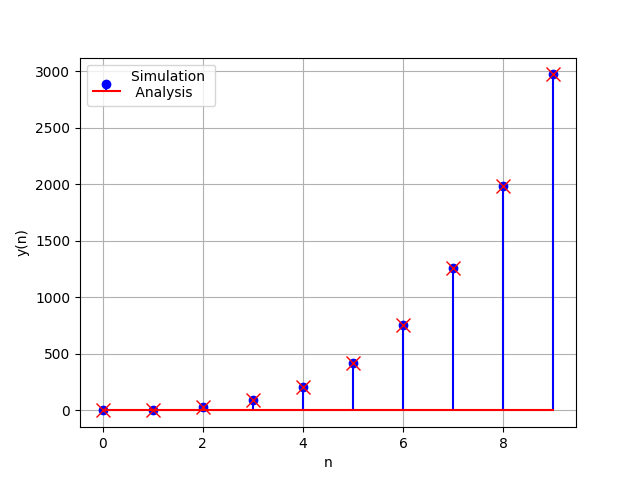
\includegraphics[width=\columnwidth]{figs/fig7.png}
    \label{fig: 10.5.3.12}
\end{figure}
\end{document}	
\pagebreak
\item  Find the sum of the following series up to \(n\) terms:
          \begin{enumerate}
              \item $5 + 55 + 555 + \ldots$
              \item  $.6 + .66 + .666 + \ldots$
        \end{enumerate}

\solution
\iffalse
\documentclass[journal,12pt,twocolumn]{IEEEtran}
\usepackage{cite}
\usepackage{amsmath,amssymb,amsfonts,amsthm,mathtools}
\usepackage{algorithmic}
\usepackage{graphicx}
\parindent 0px
\bibliographystyle{IEEEtran}
\title{NCERT DISCRETE 11.9.2 Q10}
\author{EE23BTECH11052 - Abhilash Rapolu }
\begin{document}
\maketitle
\newpage
\textbf{Question 11.9.2.10}:If the sum of first $p$ terms of an A.P. is equal to the sum of the first $q$ terms, then
find the sum of the first $(p + q)$ terms.\\
\ Solution:
\fi
\begin{table}[htbp]
\centering
\begin{tabular}{|l|l|c|}
\hline
\textbf{Parameter} & \textbf{Description} & \textbf{Value} \\
\hline
$a_0$ & first term & none \\
\hline
$d$ & common difference & none \\
\hline
$x(n)$ & $n^{th}$ term & $a_0+nd$ \\
\hline
$y(n)$ & Sum of n terms  & $\frac{n+1}{2}[2a_0+nd]$ \\
\hline
$y(p-1)$ & sum of first p terms & $\frac{p}{2}[2a_0+(p-1)d]$ \\
\hline
$y(q-1)$ & sum of first q terms & $\frac{q}{2}[2a_0+(q-1)d]$ \\
\hline
$y(p+q-1)$ & sum of first p+q terms & $\frac{p+q}{2}[2a_0+(p+q-1)d]$ \\
\hline
\end{tabular}


\caption{Given parameters list}
\end{table}
Now let's find the z transform of the $x(n)$ using the linearity property.\\
\begin{align}
X(z)&=\frac{a_0}{1-z^{-1}}+d\frac{z^{-1}}{(1-z^{-1})^2}\\
y(n) &= x(n)*u(n)
\end{align}
Now apply z transform on both sides\\
\begin{align}
Y(z)&=X(z)U(z)\\
Y(z)&=\frac{a_0}{(1-z^{-1})^2}+d\frac{z^{-1}}{(1-z^{-1})^3}
\end{align}
by comparison of the above equations:\\
using equations from appendix  \eqref{eq:uzder-shift} and \eqref{eq:uzder-der}\\
the inverse z transform:\\
\begin{align}
y(n)&=[a_0(n)+\frac{d}{2}(n)(n-1)]u(n)
\end{align}
as we considered n=0 as our first term, we have to replace n by (n+1)\\
Sum of first n terms is given as:\\
\begin{align}
y(n)&=[a_0(n+1)+\frac{d}{2}(n+1)(n)]u(n)
\end{align}
given in question y(p-1)=y(q-1)\\
\begin{align}
[a_0(p)+\frac{d}{2}(p-1)(p)]u(n)&=[a_0(q)+\frac{d}{2}(q-1)(q)]u(n)\\
d&=(-)\frac{2a_0}{p+q-1}
\end{align}
now for first p+q terms:\\
\begin{align}
y(p+q-1)&=[a_0(p+q)+\frac{d}{2}(p+q-1)(p+q)]u(n)
\end{align}
substitue d in this\\
\begin{align}
y(p+q-1)&=[a_0(p+q)-\frac{a_0}{p+q-1}(p+q-1)(p+q)]u(n)\\
y(p+q-1)&=[a_0(p+q)-a_0(p+q)]u(n)\\
y(p+q-1)&=0.
\end{align}

%\end{document}


\pagebreak
\item Find $a_{9}$ in the sequence $a_{n}=\brak{-1}^{n-1}n^{3}$ \\
\solution
\iffalse
\let\negmedspace\undefined
\let\negthickspace\undefined
\documentclass[journal,12pt,twocolumn]{IEEEtran}
\usepackage{cite}
\usepackage{amsmath,amssymb,amsfonts,amsthm}
\usepackage{algorithmic}
\usepackage{graphicx}
\usepackage{textcomp}
\usepackage{xcolor}
\usepackage{txfonts}
\usepackage{listings}
\usepackage{enumitem}
\usepackage{mathtools}
\usepackage{gensymb}
\usepackage{comment}
\usepackage[breaklinks=true]{hyperref}
\usepackage{tkz-euclide} 
\usepackage{listings}
\usepackage{gvv}                                        
\def\inputGnumericTable{}                                 
\usepackage[latin1]{inputenc}                                
\usepackage{color}                                            
\usepackage{array}                                            
\usepackage{longtable}                                       
\usepackage{calc}                                             
\usepackage{multirow}                                         
\usepackage{hhline}                                           
\usepackage{ifthen}                                           
\usepackage{lscape}


\newtheorem{theorem}{Theorem}[section]
\newtheorem{problem}{Problem}
\newtheorem{proposition}{Proposition}[section]
\newtheorem{lemma}{Lemma}[section]
\newtheorem{corollary}[theorem]{Corollary}
\newtheorem{example}{Example}[section]
\newtheorem{definition}[problem]{Definition}
\newcommand{\BEQA}{\begin{eqnarray}}
\newcommand{\EEQA}{\end{eqnarray}}
\newcommand{\define}{\stackrel{\triangle}{=}}
\theoremstyle{remark}
\newtheorem{rem}{Remark}
\begin{document}
\parindent 0px
\bibliographystyle{IEEEtran}

\title{Assignment\\[1ex]11.9.1 - 9}
\author{EE23BTECH11220 - R.V.S.S Varun$^{}$% <-this % stops a space
}
\maketitle
\newpage
\bigskip

\renewcommand{\thefigure}{\theenumi}
\renewcommand{\thetable}{\theenumi}
\section*{Question}
Find $a_{9}$ in the sequence $a_{n}=\brak{-1}^{n-1}n^{3}$ 
\fi
 
\begin{table}[h]
    \centering
    \begin{tabular}{|c|c|c|}
    \hline
	 Symbol &Value&Description \\
        \hline
	 x\brak{0}&1&First term of the sequence\\
         \hline
	 x\brak{n}&$\brak{-1}^{n}\brak{n+1}^3u\brak{n}$& $\brak{n+1}^{th}$ term of the sequence \\
         \hline
         
    \end{tabular}

    
    \caption{Table of parameters}
    \label{tab:11.9.1.9.1}
\end{table}


To obtain $9^{th}$ term of the sequence put $n$=8 in x\brak{n}
\begin{align}
x\brak{8}=729
\end{align}
Using $Z$ transform,
\begin{align}
	X\brak{z}&=\sum_{n=-\infty}^{\infty}\brak{-1}^n\brak{n+1}^3u\brak{n}z^{-n}\\
	&=\sum_{n=-\infty}^{\infty}\brak{n+1}^3u\brak{n}\brak{-z}^{-n}\\
	&=\sum_{n=-\infty}^{\infty}\brak{n^3+3n^2+3n+1}u\brak{n}\brak{-z}^{-n}
\end{align}
Replace $z$ by $-z$ in \eqref{eq:uz},\eqref{eq:11.9.5.26.2},\eqref{eq:11.9.5.26.3},\eqref{eq:11.9.5.26.4}
\begin{align}
	u\brak{n}\xleftrightarrow{\mathcal{Z}}\frac{1}{1+z^{-1}},\abs{z}>1\\
	nu\brak{n}\xleftrightarrow{\mathcal{Z}}\frac{-z^{-1}}{\brak{1+z^{-1}}^2},\abs{z}>1\\
	n^2u\brak{n}\xleftrightarrow{\mathcal{Z}}\frac{z^{-1}\brak{z^{-1}-1}}{\brak{1+z^{-1}}^3},\abs{z}>1\\
	n^3u\brak{n}\xleftrightarrow{\mathcal{Z}}\frac{-z^{-1}\brak{1-4z^{-1}+z^{-2}}}{\brak{1+z^{-1}}^4},\abs{z}>1
\end{align}

\begin{align}
	X\brak{z}=\frac{z^{-2}-z^{-1}+1}{\brak{1+z^{-1}}^4},\abs{z}>1
\end{align}

\begin{figure}[h]
    \centering
    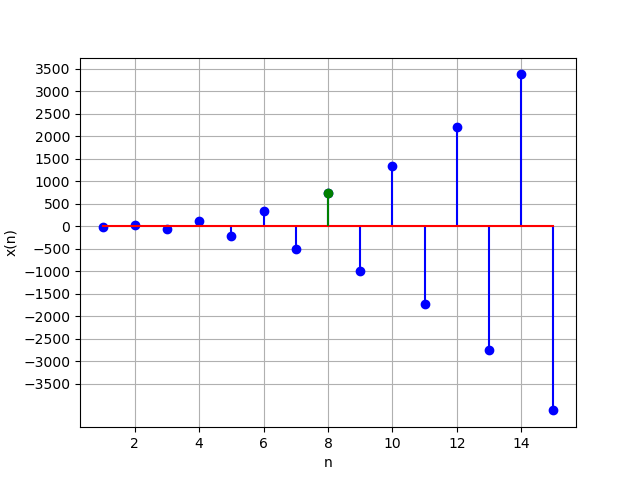
\includegraphics[width=1 \columnwidth]{ncert-maths/11/9/1/9/figs/graph.png} 
    \label{fig:11.9.1.9.1}
\end{figure}



\pagebreak


\item Q10) The sum of three numbers in G.P. is 56. If we subtract 1, 7, 21 from these numbers in that order, we obtain an arithmetic progression. Find the numbers.\\
\solution \input{ncert-maths/11/9/5/10/latexcode,discrete_seq.tex}
\pagebreak
\item  Find the sum to n terms for the given series: $3\times8 + 6\times11 + 9\times14 + ...$ \\
\solution 
 \iffalse
\let\negmedspace\undefined
\let\negthickspace\undefined
\documentclass[journal,12pt,twocolumn]{IEEEtran}
\usepackage{amssymb}
\usepackage{cite}
\usepackage{amsmath,amssymb,amsfonts,amsthm}
\usepackage{algorithmic}
\usepackage{graphicx}
\usepackage{textcomp}
\usepackage{xcolor}
\usepackage{txfonts}
\usepackage{listings}
\usepackage{enumitem}
\usepackage{mathtools}
\usepackage{gensymb}
\usepackage{comment}
\usepackage[breaklinks=true]{hyperref}
\usepackage{tkz-euclide} 
\usepackage{listings}
\usepackage{gvv}                                        
\def\inputGnumericTable{}                                 
\usepackage[latin1]{inputenc}                                
\usepackage{color}                                            
\usepackage{array}                                            
\usepackage{longtable}                                       
\usepackage{calc}                                             
\usepackage{multirow}                                         
\usepackage{hhline}                                           
\usepackage{ifthen}                                           
\usepackage{lscape}
\usepackage{pgfplots}
\newtheorem{theorem}{Theorem}[section]
\newtheorem{problem}{Problem}
\newtheorem{proposition}{Proposition}[section]
\newtheorem{lemma}{Lemma}[section]
\newtheorem{corollary}[theorem]{Corollary}
\newtheorem{example}{Example}[section]
\newtheorem{definition}[problem]{Definition}
\newcommand{\BEQA}{\begin{eqnarray}}
\newcommand{\EEQA}{\end{eqnarray}}
\newcommand{\define}{\stackrel{\triangle}{=}}
\theoremstyle{remark}
\newtheorem{rem}{Remark}
\begin{document}

\bibliographystyle{IEEEtran}
\vspace{3cm}

\title{NCERT Discrete-11.9.4-5}
\author{EE22BTECH11004 - Allu Lohith}

\maketitle
\newpage
\bigskip


 Find the sum of n terms of this sequence:$$5^2+6^2+7^2...+20^2$$  
\solution
\fi
\begin{table}[h!]
\centering
\renewcommand{\arraystretch}{2}
\begin{tabular}{|c|p{4cm}|c|}
\hline 
\setlength{\tabcolsep}{1pt}
\textbf{Parameter}  &\textbf{Description} &\textbf{Formulae/Value} \\
\hline
n & Iteration number starting from zero till 15 & - \\
\hline
$x\brak n$ & General term of the sequence from $n=0$ to $n=15$ &$\brak{n+5}^2$  u\brak n\\
\hline
$x\brak 0$ & First term of the sequence & 5 \\
\hline
\end{tabular}

\vspace{0.5cm}
\caption{\normalsize Parameters}
\end{table}
The standard $z$ transforms,
\begin{align}
    u \brak n &\stackrel{z}{\longleftrightarrow} \frac{1}{1-z^{-1}}, \abs z >1\\
   n u\brak n &\stackrel{z}{\longleftrightarrow} \frac{z^{-1}}{\brak{1-z^{-1}}^2}, \abs z >1\\
   n^2 u\brak n &\stackrel{z}{\longleftrightarrow} \frac{z^{-1}\brak{1+z^{-1}}}{\brak{1-z^{-1}}^3}, \abs z >1
\end{align}
As 
\begin{align}
    x\brak n = \brak{n^2+10n+25}u\brak n
\end{align}
The $z$ transform of general term can be written as , 
\begin{align}
    X\brak z &= \frac{z^{-1}\brak{1+z^{-1}}}{\brak{1-z^{-1}}^3}+10\frac{z^{-1}}{\brak{1-z^{-1}}^2}+\frac{25}{1-z^{-1}} \\
    X\brak z &=  \frac{16z^{-2}-39z^{-1}+25}{\brak{1-z^{-1}}^3}; \abs{z}>1
\end{align}
On convolution for finding the sum
\begin{align}
    y\brak n= x\brak n \ast u\brak n
\end{align}
On z transform,
\begin{align}
    Y\brak z &= X \brak z \cdot U \brak z\\
    &= \brak{\frac{16z^{-2}-39z^{-1}+25}{\brak{1-z^{-1}})^3}} \cdot \frac{1}{1-z^{-1}}\\
    \implies 
    Y \brak z & = \frac{16z^{-2}-39z^{-1}+25}{\brak{1-z^{-1}}^4}; \quad \abs z >1
\end{align}
Using the contour integration to find the inverse $z$ transform,
\begin{align}
    y(n)&=\oint_c Y(z)\cdot z^{n-1}dz\\
    y(21)&=\oint_c \brak{\frac{16z^{-2}-39z^{-1}+25}{\brak{1-z^{-1}}^4}} z^{14}dz
\end{align}
As there are four poles from observation, so $m=4$
\begin{align}
    y\brak{21} &= \frac{1}{(m-1)!} \lim_{z \to a} \frac{d^{m-1}}{dz^{m-1}}\brak{(z-a)^mf(z)}\\
    &= \frac{1}{3!} \lim_{z \to 1} \frac{d^{3}}{dz^{3}}\brak{(z-1)^4 \frac{\brak{16z^{-2}-39z^{-1}+25}}{(1-z^{-1})^4} z^{14}}\\
    &= \frac{1}{6} \lim_{z \to 1} \frac{d^{3}}{dz^{3}}\brak{\brak{16z^{-2}-39z^{-1}+25}z^{18}}\\
    &= \frac{1}{6} \lim_{z \to 1} \frac{d^{3}}{dz^{3}}\brak{16z^{16}-39z^{17}+25z^{18}}\\
    &= \frac{1}{6}  \brak{16 \times 18 \times 17 \times 16+14 \times 17 \times 16 \times 15 }\\
    \implies y\brak{21}&=2840 
\end{align}
Hence the sum of the terms of the sequence is 2840.

\begin{figure}[h]
    \centering  

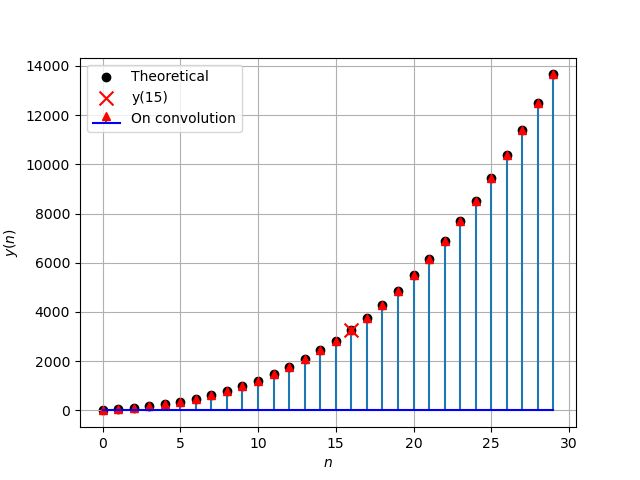
\includegraphics[width=\columnwidth]{ncert-maths/11/9/4/5/figs/plot.png}

\begin{center}
    \caption{Simulation v/s theoretical}
\end{center}
\end{figure}


\pagebreak
\item Find the sum to $n$ terms of the series:\\
$1^2+\brak{1^2+2^2}+\brak{1^2+2^2+3^2}+...$ \hfill(NCERT 11.9.4.7)\\
\solution
 \iffalse
\let\negmedspace\undefined
\let\negthickspace\undefined
\documentclass[journal,12pt,twocolumn]{IEEEtran}
\usepackage{amssymb}
\usepackage{cite}
\usepackage{amsmath,amssymb,amsfonts,amsthm}
\usepackage{algorithmic}
\usepackage{graphicx}
\usepackage{textcomp}
\usepackage{xcolor}
\usepackage{txfonts}
\usepackage{listings}
\usepackage{enumitem}
\usepackage{mathtools}
\usepackage{gensymb}
\usepackage{comment}
\usepackage[breaklinks=true]{hyperref}
\usepackage{tkz-euclide} 
\usepackage{listings}
\usepackage{gvv}                                        
\def\inputGnumericTable{}                                 
\usepackage[latin1]{inputenc}                                
\usepackage{color}                                            
\usepackage{array}                                            
\usepackage{longtable}                                       
\usepackage{calc}                                             
\usepackage{multirow}                                         
\usepackage{hhline}                                           
\usepackage{ifthen}                                           
\usepackage{lscape}
\usepackage{pgfplots}
\newtheorem{theorem}{Theorem}[section]
\newtheorem{problem}{Problem}
\newtheorem{proposition}{Proposition}[section]
\newtheorem{lemma}{Lemma}[section]
\newtheorem{corollary}[theorem]{Corollary}
\newtheorem{example}{Example}[section]
\newtheorem{definition}[problem]{Definition}
\newcommand{\BEQA}{\begin{eqnarray}}
\newcommand{\EEQA}{\end{eqnarray}}
\newcommand{\define}{\stackrel{\triangle}{=}}
\theoremstyle{remark}
\newtheorem{rem}{Remark}
\begin{document}

\bibliographystyle{IEEEtran}
\vspace{3cm}

\title{NCERT Discrete-11.9.4-5}
\author{EE22BTECH11004 - Allu Lohith}

\maketitle
\newpage
\bigskip


 Find the sum of n terms of this sequence:$$5^2+6^2+7^2...+20^2$$  
\solution
\fi
\begin{table}[h!]
\centering
\renewcommand{\arraystretch}{2}
\begin{tabular}{|c|p{4cm}|c|}
\hline 
\setlength{\tabcolsep}{1pt}
\textbf{Parameter}  &\textbf{Description} &\textbf{Formulae/Value} \\
\hline
n & Iteration number starting from zero till 15 & - \\
\hline
$x\brak n$ & General term of the sequence from $n=0$ to $n=15$ &$\brak{n+5}^2$  u\brak n\\
\hline
$x\brak 0$ & First term of the sequence & 5 \\
\hline
\end{tabular}

\vspace{0.5cm}
\caption{\normalsize Parameters}
\end{table}
The standard $z$ transforms,
\begin{align}
    u \brak n &\stackrel{z}{\longleftrightarrow} \frac{1}{1-z^{-1}}, \abs z >1\\
   n u\brak n &\stackrel{z}{\longleftrightarrow} \frac{z^{-1}}{\brak{1-z^{-1}}^2}, \abs z >1\\
   n^2 u\brak n &\stackrel{z}{\longleftrightarrow} \frac{z^{-1}\brak{1+z^{-1}}}{\brak{1-z^{-1}}^3}, \abs z >1
\end{align}
As 
\begin{align}
    x\brak n = \brak{n^2+10n+25}u\brak n
\end{align}
The $z$ transform of general term can be written as , 
\begin{align}
    X\brak z &= \frac{z^{-1}\brak{1+z^{-1}}}{\brak{1-z^{-1}}^3}+10\frac{z^{-1}}{\brak{1-z^{-1}}^2}+\frac{25}{1-z^{-1}} \\
    X\brak z &=  \frac{16z^{-2}-39z^{-1}+25}{\brak{1-z^{-1}}^3}; \abs{z}>1
\end{align}
On convolution for finding the sum
\begin{align}
    y\brak n= x\brak n \ast u\brak n
\end{align}
On z transform,
\begin{align}
    Y\brak z &= X \brak z \cdot U \brak z\\
    &= \brak{\frac{16z^{-2}-39z^{-1}+25}{\brak{1-z^{-1}})^3}} \cdot \frac{1}{1-z^{-1}}\\
    \implies 
    Y \brak z & = \frac{16z^{-2}-39z^{-1}+25}{\brak{1-z^{-1}}^4}; \quad \abs z >1
\end{align}
Using the contour integration to find the inverse $z$ transform,
\begin{align}
    y(n)&=\oint_c Y(z)\cdot z^{n-1}dz\\
    y(21)&=\oint_c \brak{\frac{16z^{-2}-39z^{-1}+25}{\brak{1-z^{-1}}^4}} z^{14}dz
\end{align}
As there are four poles from observation, so $m=4$
\begin{align}
    y\brak{21} &= \frac{1}{(m-1)!} \lim_{z \to a} \frac{d^{m-1}}{dz^{m-1}}\brak{(z-a)^mf(z)}\\
    &= \frac{1}{3!} \lim_{z \to 1} \frac{d^{3}}{dz^{3}}\brak{(z-1)^4 \frac{\brak{16z^{-2}-39z^{-1}+25}}{(1-z^{-1})^4} z^{14}}\\
    &= \frac{1}{6} \lim_{z \to 1} \frac{d^{3}}{dz^{3}}\brak{\brak{16z^{-2}-39z^{-1}+25}z^{18}}\\
    &= \frac{1}{6} \lim_{z \to 1} \frac{d^{3}}{dz^{3}}\brak{16z^{16}-39z^{17}+25z^{18}}\\
    &= \frac{1}{6}  \brak{16 \times 18 \times 17 \times 16+14 \times 17 \times 16 \times 15 }\\
    \implies y\brak{21}&=2840 
\end{align}
Hence the sum of the terms of the sequence is 2840.

\begin{figure}[h]
    \centering  

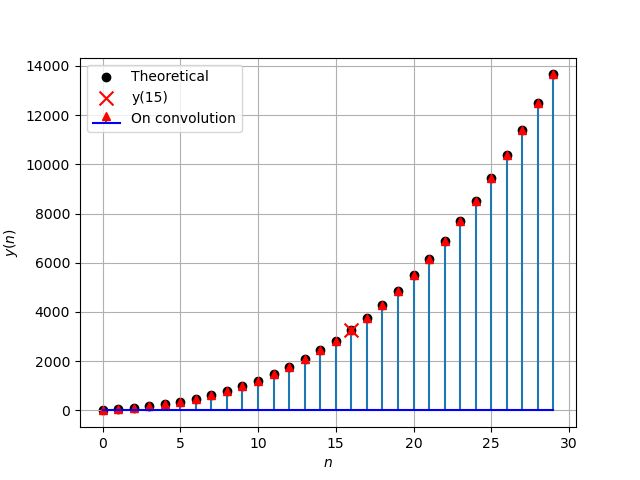
\includegraphics[width=\columnwidth]{ncert-maths/11/9/4/5/figs/plot.png}

\begin{center}
    \caption{Simulation v/s theoretical}
\end{center}
\end{figure}


\pagebreak
\item Find a GP for which sum of the first two terms is -4 and the fifth term is 4 times the third term.\\
\solution
\input{ncert-maths/11/9/3/16/question2.tex}
\pagebreak

\item Find the sum of the following series up to n terms and obtain the Z-transform: 
$$\frac{1^3}{1} + \frac{1^3 + 2^3}{1 + 3} + \frac{1^3 + 2^3 + 3^3}{1 + 3 + 5} + \ldots$$
\solution
 \iffalse
\let\negmedspace\undefined
\let\negthickspace\undefined
\documentclass[journal,12pt,twocolumn]{IEEEtran}
\usepackage{amssymb}
\usepackage{cite}
\usepackage{amsmath,amssymb,amsfonts,amsthm}
\usepackage{algorithmic}
\usepackage{graphicx}
\usepackage{textcomp}
\usepackage{xcolor}
\usepackage{txfonts}
\usepackage{listings}
\usepackage{enumitem}
\usepackage{mathtools}
\usepackage{gensymb}
\usepackage{comment}
\usepackage[breaklinks=true]{hyperref}
\usepackage{tkz-euclide} 
\usepackage{listings}
\usepackage{gvv}                                        
\def\inputGnumericTable{}                                 
\usepackage[latin1]{inputenc}                                
\usepackage{color}                                            
\usepackage{array}                                            
\usepackage{longtable}                                       
\usepackage{calc}                                             
\usepackage{multirow}                                         
\usepackage{hhline}                                           
\usepackage{ifthen}                                           
\usepackage{lscape}
\usepackage{pgfplots}
\newtheorem{theorem}{Theorem}[section]
\newtheorem{problem}{Problem}
\newtheorem{proposition}{Proposition}[section]
\newtheorem{lemma}{Lemma}[section]
\newtheorem{corollary}[theorem]{Corollary}
\newtheorem{example}{Example}[section]
\newtheorem{definition}[problem]{Definition}
\newcommand{\BEQA}{\begin{eqnarray}}
\newcommand{\EEQA}{\end{eqnarray}}
\newcommand{\define}{\stackrel{\triangle}{=}}
\theoremstyle{remark}
\newtheorem{rem}{Remark}
\begin{document}

\bibliographystyle{IEEEtran}
\vspace{3cm}

\title{NCERT Discrete-11.9.4-5}
\author{EE22BTECH11004 - Allu Lohith}

\maketitle
\newpage
\bigskip


 Find the sum of n terms of this sequence:$$5^2+6^2+7^2...+20^2$$  
\solution
\fi
\begin{table}[h!]
\centering
\renewcommand{\arraystretch}{2}
\begin{tabular}{|c|p{4cm}|c|}
\hline 
\setlength{\tabcolsep}{1pt}
\textbf{Parameter}  &\textbf{Description} &\textbf{Formulae/Value} \\
\hline
n & Iteration number starting from zero till 15 & - \\
\hline
$x\brak n$ & General term of the sequence from $n=0$ to $n=15$ &$\brak{n+5}^2$  u\brak n\\
\hline
$x\brak 0$ & First term of the sequence & 5 \\
\hline
\end{tabular}

\vspace{0.5cm}
\caption{\normalsize Parameters}
\end{table}
The standard $z$ transforms,
\begin{align}
    u \brak n &\stackrel{z}{\longleftrightarrow} \frac{1}{1-z^{-1}}, \abs z >1\\
   n u\brak n &\stackrel{z}{\longleftrightarrow} \frac{z^{-1}}{\brak{1-z^{-1}}^2}, \abs z >1\\
   n^2 u\brak n &\stackrel{z}{\longleftrightarrow} \frac{z^{-1}\brak{1+z^{-1}}}{\brak{1-z^{-1}}^3}, \abs z >1
\end{align}
As 
\begin{align}
    x\brak n = \brak{n^2+10n+25}u\brak n
\end{align}
The $z$ transform of general term can be written as , 
\begin{align}
    X\brak z &= \frac{z^{-1}\brak{1+z^{-1}}}{\brak{1-z^{-1}}^3}+10\frac{z^{-1}}{\brak{1-z^{-1}}^2}+\frac{25}{1-z^{-1}} \\
    X\brak z &=  \frac{16z^{-2}-39z^{-1}+25}{\brak{1-z^{-1}}^3}; \abs{z}>1
\end{align}
On convolution for finding the sum
\begin{align}
    y\brak n= x\brak n \ast u\brak n
\end{align}
On z transform,
\begin{align}
    Y\brak z &= X \brak z \cdot U \brak z\\
    &= \brak{\frac{16z^{-2}-39z^{-1}+25}{\brak{1-z^{-1}})^3}} \cdot \frac{1}{1-z^{-1}}\\
    \implies 
    Y \brak z & = \frac{16z^{-2}-39z^{-1}+25}{\brak{1-z^{-1}}^4}; \quad \abs z >1
\end{align}
Using the contour integration to find the inverse $z$ transform,
\begin{align}
    y(n)&=\oint_c Y(z)\cdot z^{n-1}dz\\
    y(21)&=\oint_c \brak{\frac{16z^{-2}-39z^{-1}+25}{\brak{1-z^{-1}}^4}} z^{14}dz
\end{align}
As there are four poles from observation, so $m=4$
\begin{align}
    y\brak{21} &= \frac{1}{(m-1)!} \lim_{z \to a} \frac{d^{m-1}}{dz^{m-1}}\brak{(z-a)^mf(z)}\\
    &= \frac{1}{3!} \lim_{z \to 1} \frac{d^{3}}{dz^{3}}\brak{(z-1)^4 \frac{\brak{16z^{-2}-39z^{-1}+25}}{(1-z^{-1})^4} z^{14}}\\
    &= \frac{1}{6} \lim_{z \to 1} \frac{d^{3}}{dz^{3}}\brak{\brak{16z^{-2}-39z^{-1}+25}z^{18}}\\
    &= \frac{1}{6} \lim_{z \to 1} \frac{d^{3}}{dz^{3}}\brak{16z^{16}-39z^{17}+25z^{18}}\\
    &= \frac{1}{6}  \brak{16 \times 18 \times 17 \times 16+14 \times 17 \times 16 \times 15 }\\
    \implies y\brak{21}&=2840 
\end{align}
Hence the sum of the terms of the sequence is 2840.

\begin{figure}[h]
    \centering  

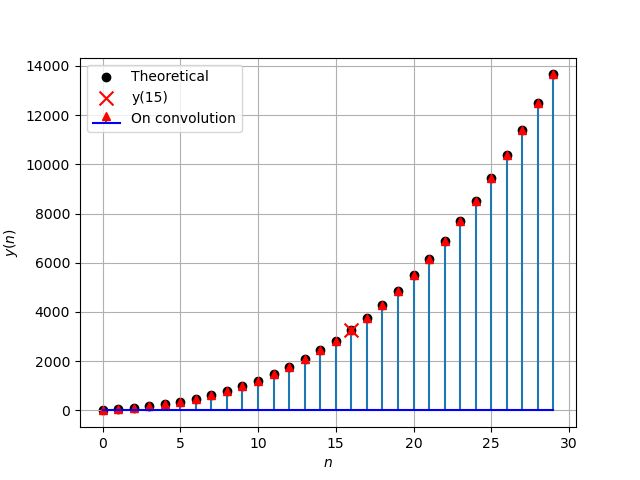
\includegraphics[width=\columnwidth]{ncert-maths/11/9/4/5/figs/plot.png}

\begin{center}
    \caption{Simulation v/s theoretical}
\end{center}
\end{figure}


\pagebreak
\item Insert five numbers between 8 and 26 such that the resulting sequence is an A.P. and obtain the Z-transform of the sequence. \\
\solution
 \iffalse
\let\negmedspace\undefined
\let\negthickspace\undefined
\documentclass[journal,12pt,twocolumn]{IEEEtran}
\usepackage{amssymb}
\usepackage{cite}
\usepackage{amsmath,amssymb,amsfonts,amsthm}
\usepackage{algorithmic}
\usepackage{graphicx}
\usepackage{textcomp}
\usepackage{xcolor}
\usepackage{txfonts}
\usepackage{listings}
\usepackage{enumitem}
\usepackage{mathtools}
\usepackage{gensymb}
\usepackage{comment}
\usepackage[breaklinks=true]{hyperref}
\usepackage{tkz-euclide} 
\usepackage{listings}
\usepackage{gvv}                                        
\def\inputGnumericTable{}                                 
\usepackage[latin1]{inputenc}                                
\usepackage{color}                                            
\usepackage{array}                                            
\usepackage{longtable}                                       
\usepackage{calc}                                             
\usepackage{multirow}                                         
\usepackage{hhline}                                           
\usepackage{ifthen}                                           
\usepackage{lscape}
\usepackage{pgfplots}
\newtheorem{theorem}{Theorem}[section]
\newtheorem{problem}{Problem}
\newtheorem{proposition}{Proposition}[section]
\newtheorem{lemma}{Lemma}[section]
\newtheorem{corollary}[theorem]{Corollary}
\newtheorem{example}{Example}[section]
\newtheorem{definition}[problem]{Definition}
\newcommand{\BEQA}{\begin{eqnarray}}
\newcommand{\EEQA}{\end{eqnarray}}
\newcommand{\define}{\stackrel{\triangle}{=}}
\theoremstyle{remark}
\newtheorem{rem}{Remark}
\begin{document}

\bibliographystyle{IEEEtran}
\vspace{3cm}

\title{NCERT Discrete-11.9.4-5}
\author{EE22BTECH11004 - Allu Lohith}

\maketitle
\newpage
\bigskip


 Find the sum of n terms of this sequence:$$5^2+6^2+7^2...+20^2$$  
\solution
\fi
\begin{table}[h!]
\centering
\renewcommand{\arraystretch}{2}
\begin{tabular}{|c|p{4cm}|c|}
\hline 
\setlength{\tabcolsep}{1pt}
\textbf{Parameter}  &\textbf{Description} &\textbf{Formulae/Value} \\
\hline
n & Iteration number starting from zero till 15 & - \\
\hline
$x\brak n$ & General term of the sequence from $n=0$ to $n=15$ &$\brak{n+5}^2$  u\brak n\\
\hline
$x\brak 0$ & First term of the sequence & 5 \\
\hline
\end{tabular}

\vspace{0.5cm}
\caption{\normalsize Parameters}
\end{table}
The standard $z$ transforms,
\begin{align}
    u \brak n &\stackrel{z}{\longleftrightarrow} \frac{1}{1-z^{-1}}, \abs z >1\\
   n u\brak n &\stackrel{z}{\longleftrightarrow} \frac{z^{-1}}{\brak{1-z^{-1}}^2}, \abs z >1\\
   n^2 u\brak n &\stackrel{z}{\longleftrightarrow} \frac{z^{-1}\brak{1+z^{-1}}}{\brak{1-z^{-1}}^3}, \abs z >1
\end{align}
As 
\begin{align}
    x\brak n = \brak{n^2+10n+25}u\brak n
\end{align}
The $z$ transform of general term can be written as , 
\begin{align}
    X\brak z &= \frac{z^{-1}\brak{1+z^{-1}}}{\brak{1-z^{-1}}^3}+10\frac{z^{-1}}{\brak{1-z^{-1}}^2}+\frac{25}{1-z^{-1}} \\
    X\brak z &=  \frac{16z^{-2}-39z^{-1}+25}{\brak{1-z^{-1}}^3}; \abs{z}>1
\end{align}
On convolution for finding the sum
\begin{align}
    y\brak n= x\brak n \ast u\brak n
\end{align}
On z transform,
\begin{align}
    Y\brak z &= X \brak z \cdot U \brak z\\
    &= \brak{\frac{16z^{-2}-39z^{-1}+25}{\brak{1-z^{-1}})^3}} \cdot \frac{1}{1-z^{-1}}\\
    \implies 
    Y \brak z & = \frac{16z^{-2}-39z^{-1}+25}{\brak{1-z^{-1}}^4}; \quad \abs z >1
\end{align}
Using the contour integration to find the inverse $z$ transform,
\begin{align}
    y(n)&=\oint_c Y(z)\cdot z^{n-1}dz\\
    y(21)&=\oint_c \brak{\frac{16z^{-2}-39z^{-1}+25}{\brak{1-z^{-1}}^4}} z^{14}dz
\end{align}
As there are four poles from observation, so $m=4$
\begin{align}
    y\brak{21} &= \frac{1}{(m-1)!} \lim_{z \to a} \frac{d^{m-1}}{dz^{m-1}}\brak{(z-a)^mf(z)}\\
    &= \frac{1}{3!} \lim_{z \to 1} \frac{d^{3}}{dz^{3}}\brak{(z-1)^4 \frac{\brak{16z^{-2}-39z^{-1}+25}}{(1-z^{-1})^4} z^{14}}\\
    &= \frac{1}{6} \lim_{z \to 1} \frac{d^{3}}{dz^{3}}\brak{\brak{16z^{-2}-39z^{-1}+25}z^{18}}\\
    &= \frac{1}{6} \lim_{z \to 1} \frac{d^{3}}{dz^{3}}\brak{16z^{16}-39z^{17}+25z^{18}}\\
    &= \frac{1}{6}  \brak{16 \times 18 \times 17 \times 16+14 \times 17 \times 16 \times 15 }\\
    \implies y\brak{21}&=2840 
\end{align}
Hence the sum of the terms of the sequence is 2840.

\begin{figure}[h]
    \centering  

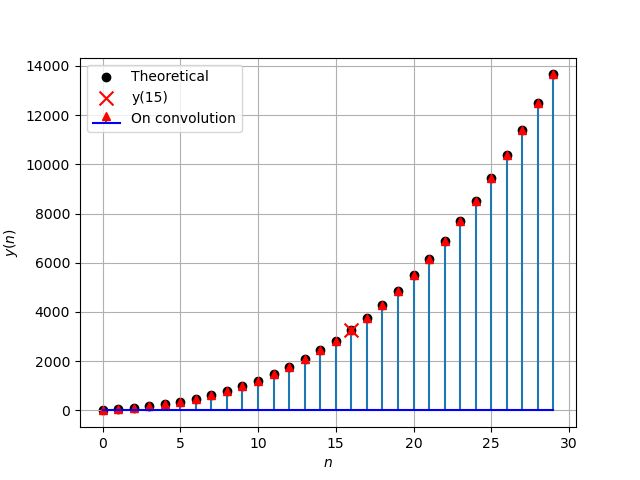
\includegraphics[width=\columnwidth]{ncert-maths/11/9/4/5/figs/plot.png}

\begin{center}
    \caption{Simulation v/s theoretical}
\end{center}
\end{figure}


\pagebreak

\item If \(S_1\), \(S_2\), \(S_3\) are the sum of the first \(n\) natural numbers, their squares, and their cubes, respectively, show that 
\[ 9(S_2)^2 = (S_3)(1 + 8(S_1)) \]\\
\solution
\let\negthickspace\undefined
\documentclass[journal,12pt,onecolumn]{IEEEtran}
\usepackage{cite}
\usepackage{amsmath,amssymb,amsfonts,amsthm}
\usepackage{algorithmic}
\usepackage{graphicx}
\usepackage{textcomp}
\usepackage{xcolor}
\usepackage{txfonts}
\usepackage{listings}
\usepackage{enumitem}
\usepackage{mathtools}
\usepackage{gensymb}

\usepackage{tkz-euclide} % loads  TikZ and tkz-base
\usepackage{listings}



\newtheorem{theorem}{Theorem}[section]
\newtheorem{problem}{Problem}
\newtheorem{proposition}{Proposition}[section]
\newtheorem{lemma}{Lemma}[section]
\newtheorem{corollary}[theorem]{Corollary}
\newtheorem{example}{Example}[section]
\newtheorem{definition}[problem]{Definition}
%\newtheorem{thm}{Theorem}[section] 
%\newtheorem{defn}[thm]{Definition}
%\newtheorem{algorithm}{Algorithm}[section]
%\newtheorem{cor}{Corollary}
\newcommand{\BEQA}{\begin{eqnarray}}
\newcommand{\EEQA}{\end{eqnarray}}
\newcommand{\system}[1]{\stackrel{#1}{\rightarrow}}

\newcommand{\define}{\stackrel{\triangle}{=}}
\theoremstyle{remark}
\newtheorem{rem}{Remark}
%\bibliographystyle{ieeetr}
\begin{document}
%
\providecommand{\pr}[1]{\ensuremath{\Pr\left(#1\right)}}
\providecommand{\prt}[2]{\ensuremath{p_{#1}^{\left(#2\right)} }}        % own macro for this question
\providecommand{\qfunc}[1]{\ensuremath{Q\left(#1\right)}}
\providecommand{\sbrak}[1]{\ensuremath{{}\left[#1\right]}}
\newcommand{\brac}[1]{\left( #1 \right)}
\providecommand{\lsbrak}[1]{\ensuremath{{}\left[#1\right.}}
\providecommand{\rsbrak}[1]{\ensuremath{{}\left.#1\right]}}
\providecommand{\brak}[1]{\ensuremath{\left(#1\right)}}
\providecommand{\lbrak}[1]{\ensuremath{\left(#1\right.}}
\providecommand{\rbrak}[1]{\ensuremath{\left.#1\right)}}
\providecommand{\cbrak}[1]{\ensuremath{\left\{#1\right\}}}
\providecommand{\lcbrak}[1]{\ensuremath{\left\{#1\right.}}
\providecommand{\rcbrak}[1]{\ensuremath{\left.#1\right\}}}
\newcommand{\sgn}{\mathop{\mathrm{sgn}}}
\providecommand{\abs}[1]{\left\vert#1\right\vert}
\providecommand{\res}[1]{\Res\displaylimits_{#1}} 
\providecommand{\norm}[1]{\left\lVert#1\right\rVert}
%\providecommand{\norm}[1]{\lVert#1\rVert}
\providecommand{\mtx}[1]{\mathbf{#1}}
\providecommand{\mean}[1]{E\left[ #1 \right]}
\providecommand{\cond}[2]{#1\middle|#2}
\providecommand{\fourier}{\overset{\mathcal{F}}{ \rightleftharpoons}}
\newenvironment{amatrix}[1]{%
  \left(\begin{array}{@{}*{#1}{c}|c@{}}
}{%
  \end{array}\right)
}
%\providecommand{\hilbert}{\overset{\mathcal{H}}{ \rightleftharpoons}}
%\providecommand{\system}{\overset{\mathcal{H}}{ \longleftrightarrow}}
    %\newcommand{\solution}[2]{\textbf{Solution:}{#1}}
\newcommand{\solution}{\noindent \textbf{Solution: }}
\newcommand{\cosec}{\,\text{cosec}\,}
\providecommand{\dec}[2]{\ensuremath{\overset{#1}{\underset{#2}{\gtrless}}}}
\newcommand{\myvec}[1]{\ensuremath{\begin{pmatrix}#1\end{pmatrix}}}
\newcommand{\mydet}[1]{\ensuremath{\begin{vmatrix}#1\end{vmatrix}}}
\newcommand{\myaugvec}[2]{\ensuremath{\begin{amatrix}{#1}#2\end{amatrix}}}
\providecommand{\rank}{\text{rank}}
\providecommand{\pr}[1]{\ensuremath{\Pr\left(#1\right)}}
\providecommand{\qfunc}[1]{\ensuremath{Q\left(#1\right)}}
    \newcommand*{\permcomb}[4][0mu]{{{}^{#3}\mkern#1#2_{#4}}}
\newcommand*{\perm}[1][-3mu]{\permcomb[#1]{P}}
\newcommand*{\comb}[1][-1mu]{\permcomb[#1]{C}}
\providecommand{\qfunc}[1]{\ensuremath{Q\left(#1\right)}}
\providecommand{\gauss}[2]{\mathcal{N}\ensuremath{\left(#1,#2\right)}}
\providecommand{\diff}[2]{\ensuremath{\frac{d{#1}}{d{#2}}}}
\providecommand{\myceil}[1]{\left \lceil #1 \right \rceil }
\newcommand\figref{Fig.~\ref}
\newcommand\tabref{Table~\ref}
\newcommand{\sinc}{\,\text{sinc}\,}
\newcommand{\rect}{\,\text{rect}\,}
%%
%   %\newcommand{\solution}[2]{\textbf{Solution:}{#1}}
%\newcommand{\solution}{\noindent \textbf{Solution: }}
%\newcommand{\cosec}{\,\text{cosec}\,}
%\numberwithin{equation}{section}
%\numberwithin{equation}{subsection}
%\numberwithin{problem}{section}
%\numberwithin{definition}{section}
%\makeatletter
%\@addtoreset{figure}{problem}
%\makeatother

%\let\StandardTheFigure\thefigure
\let\vec\mathbf


\bibliographystyle{IEEEtran}
\title{Discreet 12.9.5.24}
\author{HIBA MUHAMMED\\
        EE23BTECH11026}
\maketitle

\section*{Problem Statement}
If \(S_1\), \(S_2\), \(S_3\) are the sum of the first \(n\) natural numbers, their squares, and their cubes, respectively, show that 
\[ 9(S\scriptstyle 2)^2 = (S\scriptstyle 3)(1 + 8(S\scriptstyle 1)) \]

\section*{Solution}
\begin{table}[h]
  \centering
  \begin{tabular}{|c|c|c|}
    \hline
    \textbf{Sequence} & \textbf{Expression} & \textbf{Description} \\
    \hline
    \(s_1\) & \(\frac{n(n+1)}{2}\) & sum of n natural numbers\\
    \hline
    \(s_2\) & \(\frac{n(n+1)(2n+1)}{6}\) & sum of squares\\
    \hline
    \(s_3\) & \(\left(\frac{n(n+1)}{2}\right)^2\) & sum of cubes \\
    \hline
    \(x_1\) & \(x_1\brak{n} = n u\brak{n}\) & \\
    \hline
    \(x_2\) & \(x_2\brak{n} = n^2 u\brak{n}\) &  \\
    \hline
    \(x_3\) & \(x_3\brak{n} = n^3 u\brak{n}\) & \\
    \hline
\end{tabular}


  \caption{Input Equations}
  \label{tab:input-equations}
\end{table}
\begin{align}
    n u(n) & \xleftrightarrow{\mathcal{Z}} \frac{z^{-1}}{(1-z^{-1})^2},  \quad \abs{z} > 1 &\label{eq:12.9.5.24.1} \\
    n^2 u(n) & \xleftrightarrow{\mathcal{Z}} \frac{z^{-1}(z^{-1}+1)}{(1-z^{-1})^3},  \quad \abs{z} > 1 &\label{eq:12.9.5.24.2} \\
    n^3 u(n) & \xleftrightarrow{\mathcal{Z}} \frac{z^{-1}(1+4z^{-1}+z^{-2})}{(1-z^{-1})^4},  \quad \abs{z} >1  &\label{eq:12.9.5.24.3} \\
    n^4 u(n) & \xleftrightarrow{\mathcal{Z}} \frac{z^{-1}(1+11z^{-1}+11z^{-2}+z^{-3})}{(1-z^{-1})^5} &\label{eq:12.9.5.24.4} \\
    x(n) & \xleftrightarrow{\mathcal{Z}} X(z) \label{eq:12.9.5.24.5} \\
    y(x) &= x(n)* u(n) \label{eq:12.9.5.24.6} \\
    Y(z) &= X(z) \cdot u(z)  \label{eq:12.9.5.24.7} 
\end{align}
from \eqref{eq:12.9.5.24.1} to \eqref{eq:12.9.5.24.7}  \\
    \begin{enumerate}
    \item 
    \begin{align}
    X_1(z) &= \frac{z^{-1}}{(1-z^{-1})^2},  \quad |z| > 1 \\
    Y_1(z) &= \frac{z^{-1}}{(1-z^{-1})^3} \\
    Y_1(z) &= \frac{-1}{(1-z^{-1})^2}+\frac{1}{(1-z^{-1})^3} \\
    y_1(n) &= n\frac{(n+1)}{2}u(n)\\
    \end{align}
    \item
    \begin{align} 
    X_2(z) &= \frac{z^{-1}(z^{-1}+1)}{(1-z^{-1})^3},  \quad |z| > 1 \\
    Y_2(z) &= \frac{z^{-1}(z^{-1}+1)}{(1-z^{-1})^4} \\ 
    Y_2(z) &= \frac{1}{(1-z^{-1})^2}-\frac{3}{(1-z^{-1})^3}+\frac{2}{(1-z^{-1})^4} \\
    y_2(n) &= \frac{(n)(n+1)(2n+1)}{6}u(n) \\
    \end{align}
    \item 
    \begin{align}
    X_3(z) &= \frac{z^{-1}(1+4z^{-1}+z^{-2})}{(1-z^{-1})^4},  \quad |z| > 1 \\
    Y_3(z) &= \frac{z^{-1}(1+4z^{-1}+z^{-2})}{(1-z^{-1})^5}\\
    Y_3(z) &= \frac{-1}{(1-z^{-1})^2}+\frac{7}{(1-z^{-1})^3}-\frac{12}{(1-z^{-1})^4}+\frac{6}{(1-z^{-1})^5}\\
    y_3(n) &= \left(\frac{(n)(n+1)}{2}\right)^2u(n)
    \end{align}
    \end{enumerate}
$y_2^2 = (y_3)(1 + 8(y_1))$ 
\begin{align}
\text{LHS} &= 9(y_2)^2 = 9\left(\frac{(n+1)(n)(2n+1)}{6}\right)^2u(n)\\
&=n^6 u(n)^2 + 3n^5 u(n)^2 + \frac{13}{4}n^4 u(n)^2 + \frac{3}{2}n^3 u(n)^2 + \frac{1}{4}n^2 u(n)^2\\
&= n^6 + 3n^5 + \frac{13}{4}n^4 + \frac{3}{2}n^3 + \frac{1}{4}n^2 &n\geq0\\
\text{RHS} &= (y_3)(1 + 8(y_1)) = \left(\frac{(n+1)(n+2)}{2}\right)^2u(n)(1+8\left(\frac{(n+1)(n+2)}{2}\right)u(n)) \\
&=n^6 u(n)^3 + 3n^5 u(n)^3 + 3n^4 u(n)^3 + \frac{1}{4}n^4 u(n)^2 + n^3 u(n)^3 + \frac{1}{2}n^3 u(n)^2 + \frac{1}{4}n^2 u(n)^2\\
&= n^6 + 3n^5 + \frac{13}{4}n^4 + \frac{3}{2}n^3 + \frac{1}{4}n^2 &n\geq0
\end{align}

LHS=RHS
\[ 9(S_2)^2 = (S_3)(1 + 8(S_1)) \]
\begin{figure}[htbp]
    \centering
    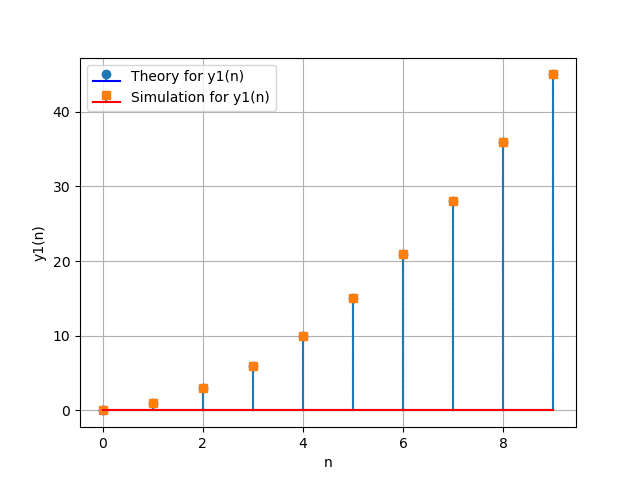
\includegraphics[width=0.5\textwidth]{figs/y_1(n).png}
    \caption{Simulation vs Theory for y1(n)}
    \label{fig:figure1}
\end{figure}  

\begin{figure}[htbp]
    \centering
    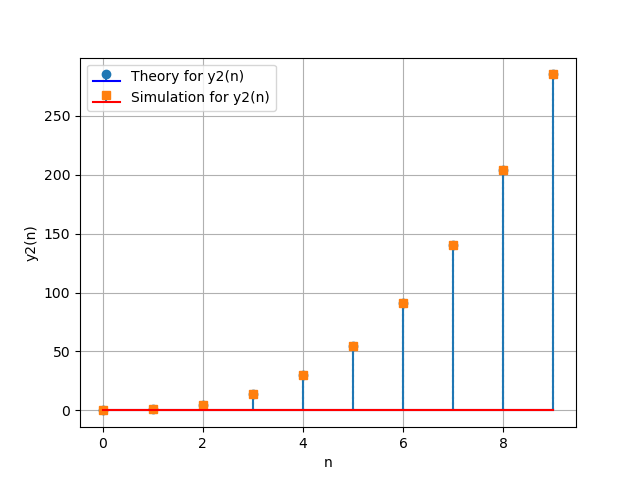
\includegraphics[width=0.5\textwidth]{figs/y_2(n).png}
    \caption{Simulation vs Theory for y2(n)}
    \label{fig:figure2}
\end{figure}   

\begin{figure}[htbp]
    \centering
    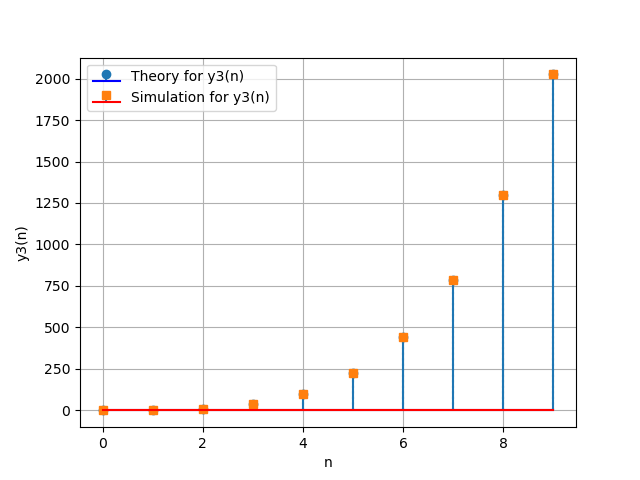
\includegraphics[width=0.5\textwidth]{figs/y_3(n).png}
    \caption{Simulation vs Theory for y3(n) }
    \label{fig:figure3}
\end{figure} 
\end{document}

\pagebreak


\item If a, b, c, d are in G.P, prove that 
$ \brak{a^{n} + b^{n}},\brak{b^{n} + c^{n}},\brak{c^{n} + d^{n}} $ are in G.P \\
\solution
\input{ncert-maths/11/9/5/17/gp.tex}
\pagebreak

\item Write the first five terms of the sequence whose $n^{th}$ terms  $a_n = \frac{n}{n+1}$\\
\solution
\input{ncert-maths/11/9/1/2/11.9.1.2.tex}
\pagebreak

\item 150 workers were engaged to finish a job in a certain number of days, 4 workers dropped out on second day, 4 more workers dropped out on third day and so on. It took 8 more days to finish the work. Find the number of days in which the work was completed.\\
\solution
\let\negmedspace\undefined
\let\negthickspace\undefined
\documentclass[a4,12pt,twocolumn]{IEEEtran}
%\documentclass[conference]{IEEEtran}
%\IEEEoverridecommandlockouts
% The preceding line is only needed to identify funding in the first footnote. If that is unneeded, please comment it out.
\usepackage{cite}
\usepackage{amsmath,amssymb,amsfonts,amsthm}
\usepackage{algorithmic}
\usepackage{graphicx}
\usepackage{textcomp}
\usepackage{xcolor}
\usepackage{txfonts}
\usepackage{listings}
\usepackage{enumitem}
\usepackage{mathtools}
\usepackage{gensymb}
\usepackage[breaklinks=true]{hyperref}
\usepackage{tkz-euclide} % loads  TikZ and tkz-base
\usepackage{listings}
\usepackage{empheq}
%
%\usepackage{setspace}
%\usepackage{gensymb}
%\doublespacing
%\singlespacing

%\usepackage{graphicx}
%\usepackage{amssymb}
%\usepackage{relsize}
%\usepackage[cmex10]{amsmath}
%\usepackage{amsthm}
%\interdisplaylinepenalty=2500
%\savesymbol{iint}
%\usepackage{txfonts}
%\restoresymbol{TXF}{iint}
%\usepackage{wasysym}
%\usepackage{amsthm}
%\usepackage{iithtlc}
%\usepackage{mathrsfs}
%\usepackage{txfonts}
%\usepackage{stfloats}
%\usepackage{bm}
%\usepackage{cite}
%\usepackage{cases}
%\usepackage{subfig}
%\usepackage{xtab}
%\usepackage{longtable}
%\usepackage{multirow}
%\usepackage{algorithm}
%\usepackage{algpseudocode}
%\usepackage{enumitem}
%\usepackage{mathtools}
%\usepackage{tikz}
%\usepackage{circuitikz}
%\usepackage{verbatim}
%\usepackage{tfrupee}
%\usepackage{stmaryrd}
%\usetkzobj{all}
%    \usepackage{color}                                            %%
\usepackage{array}                                            %%
%    \usepackage{longtable}                                        %%
%    \usepackage{calc}                                             %%
%    \usepackage{multirow}                                         %%
%    \usepackage{hhline}                                           %%
%    \usepackage{ifthen}                                           %%
  %optionally (for landscape tables embedded in another document): %%
%    \usepackage{lscape}     
%\usepackage{multicol}
%\usepackage{chngcntr}
%\usepackage{enumerate}

%\usepackage{wasysym}
%\newcounter{MYtempeqncnt}
\DeclareMathOperator*{\Res}{Res}
%\renewcommand{\baselinestretch}{2}
\renewcommand\thesection{\arabic{section}}
\renewcommand\thesubsection{\thesection.\arabic{subsection}}
\renewcommand\thesubsubsection{\thesubsection.\arabic{subsubsection}}

\renewcommand\thesectiondis{\arabic{section}}
\renewcommand\thesubsectiondis{\thesectiondis.\arabic{subsection}}
\renewcommand\thesubsubsectiondis{\thesubsectiondis.\arabic{subsubsection}}

% correct bad hyphenation here
\hyphenation{op-tical net-works semi-conduc-tor}
\def\inputGnumericTable{}                                 %%

\lstset{
%language=C,
frame=single, 
breaklines=true,
columns=fullflexible
}
%\lstset{
%language=tex,
%frame=single, 
%breaklines=true
%}

\begin{document}
%


\newtheorem{theorem}{Theorem}[section]
\newtheorem{problem}{Problem}
\newtheorem{proposition}{Proposition}[section]
\newtheorem{lemma}{Lemma}[section]
\newtheorem{corollary}[theorem]{Corollary}
\newtheorem{example}{Example}[section]
\newtheorem{definition}[problem]{Definition}
%\newtheorem{thm}{Theorem}[section] 
%\newtheorem{defn}[thm]{Definition}
%\newtheorem{algorithm}{Algorithm}[section]
%\newtheorem{cor}{Corollary}
\newcommand{\BEQA}{\begin{eqnarray}}
\newcommand{\EEQA}{\end{eqnarray}}
\newcommand{\define}{\stackrel{\triangle}{=}}

\bibliographystyle{IEEEtran}
%\bibliographystyle{ieeetr}


\providecommand{\mbf}{\mathbf}
\providecommand{\pr}[1]{\ensuremath{\Pr\left(#1\right)}}
\providecommand{\qfunc}[1]{\ensuremath{Q\left(#1\right)}}
\providecommand{\sbrak}[1]{\ensuremath{{}\left[#1\right]}}
\providecommand{\lsbrak}[1]{\ensuremath{{}\left[#1\right.}}
\providecommand{\rsbrak}[1]{\ensuremath{{}\left.#1\right]}}
\providecommand{\brak}[1]{\ensuremath{\left(#1\right)}}
\providecommand{\lbrak}[1]{\ensuremath{\left(#1\right.}}
\providecommand{\rbrak}[1]{\ensuremath{\left.#1\right)}}
\providecommand{\cbrak}[1]{\ensuremath{\left\{#1\right\}}}
\providecommand{\lcbrak}[1]{\ensuremath{\left\{#1\right.}}
\providecommand{\rcbrak}[1]{\ensuremath{\left.#1\right\}}}
\theoremstyle{remark}
\newtheorem{rem}{Remark}
\newcommand{\sgn}{\mathop{\mathrm{sgn}}}
%\providecommand{\abs}[1]{\left\vert#1\right\vert}
\providecommand{\res}[1]{\Res\displaylimits_{#1}} 
%\providecommand{\norm}[1]{\left\lVert#1\right\rVert}
%\providecommand{\norm}[1]{\lVert#1\rVert}
\providecommand{\mtx}[1]{\mathbf{#1}}
%\providecommand{\mean}[1]{E\left[ #1 \right]}
\providecommand{\fourier}{\overset{\mathcal{F}}{ \rightleftharpoons}}
%\providecommand{\hilbert}{\overset{\mathcal{H}}{ \rightleftharpoons}}
\providecommand{\system}{\overset{\mathcal{H}}{ \longleftrightarrow}}
	%\newcommand{\solution}[2]{\textbf{Solution:}{#1}}
\newcommand{\solution}{\noindent \textbf{Solution: }}
\newcommand{\cosec}{\,\text{cosec}\,}
\providecommand{\dec}[2]{\ensuremath{\overset{#1}{\underset{#2}{\gtrless}}}}
\newcommand{\myvec}[1]{\ensuremath{\begin{pmatrix}#1\end{pmatrix}}}
\newcommand{\mydet}[1]{\ensuremath{\begin{vmatrix}#1\end{vmatrix}}}
%\numberwithin{equation}{section}
%\numberwithin{equation}{subsection}
%\numberwithin{problem}{section}
%\numberwithin{definition}{section}
%\makeatletter
%\@addtoreset{figure}{problem}
%\makeatother

%\let\StandardTheFigure\thefigure
\let\vec\mathbf

\title{
\Huge\textbf{Discrete Assignment}\\
\Huge\textbf{EE1205} Signals and Systems\\
}
\large\author{Nimal Sreekumar\\EE23BTECH11044}

% make the title area
\maketitle


%\tableofcontents

\bigskip

\renewcommand{\thefigure}{\arabic{figure}}
\renewcommand{\thetable}{\theenumi}
%\renewcommand{\theequation}{\theenumi}


\textbf{Question 11.9.5.32:}
150 workers were engaged to finish a job in a certain number of days, 4 workers dropped out on second day, 4 more workers dropped out on third day and so on. It took 8 more days to finish the work. Find the number of days in which the work was completed.\\

\solution\\
\begin{tabular}{|c|c|}
	\hline
	\textbf{Parameter} & \textbf{Description} \\[6pt]
	\hline
     $R_x\brak{\tau}$ & Autocorrection factor function \\
     \hline
     $ X\brak{t}$ & Stationary random process \\
    \hline
    $ P_x$ & Average power\\
    \hline
\end{tabular}


\begin{align}
\text{Total work done} &= 150p\label{eq:11.9.5.32.1}
\end{align}
\begin{align}
x\brak{n} &= \brak{150-4n}u\brak{n}\label{eq:11.9.5.32.2}\\
X\brak{z} &= \frac{150}{1-z^{-1}}- \frac{4z^{-1}}{\brak{1-z^{-1}}^2} \qquad ,|z| > 1 \label{eq:11.9.5.32.3}\\
y\brak{n} &= x\brak{n}*u\brak{n}\label{eq:11.9.5.32.4}\\
Y\brak{z} &= X\brak{z}U\brak{z}\label{eq:11.9.5.32.5}\\
Y\brak{z} &=\frac{150}{\brak{1-z^{-1}}^2}- \frac{4z^{-1}}{\brak{1-z^{-1}}^3} \qquad ,|z| > 1\label{eq:11.9.5.32.6}
\end{align}
Using the $z$ transforms given below:
\begin{align}
\brak{n+1}u\brak{n} \xleftrightarrow{z} \frac{1}{\brak{1-z^{-1}}^2} \qquad ,|z| > 1 \label{eq:11.9.5.32.7}\\
n\brak{\brak{n+1}u\brak{n}}\xleftrightarrow{z} \frac{2z^{-1}}{\brak{1-z^{-1}}^3} \qquad ,|z| > 1 \label{eq:11.9.5.32.8}
\end{align}

\begin{align}
\implies y\brak{n} &= 150\brak{n+1}u\brak{n} - 2n\brak{\brak{n+1}u\brak{n}}\label{eq:11.9.5.32.9}\\
y\brak{n} &= \brak{148n - 2n^2 + 150}u\brak{n}\label{eq:11.9.5.32.10}
\end{align}

It takes additional 8 days to complete work
\begin{align}
\text{Total work done} = y\brak{p+7}\label{eq:11.9.5.32.11}
\end{align}

Equating \eqref{eq:11.9.5.32.1} and \eqref{eq:11.9.5.32.11}:
\begin{align}
120p - 2p^2 +1088 &= 150p\label{eq:11.9.5.32.12}\\
\brak{p-17}\brak{p+32} &= 0 \label{eq:11.9.5.32.13}\\
p &= 17 \qquad ,\brak{p\geq 0}\label{eq:11.9.5.32.14}
\end{align}
\begin{align}
\text{Work completed in} = p+8= 25 \text{days}\label{eq:11.9.5.32.15}
\end{align}

\begin{figure}[h]
\centering
   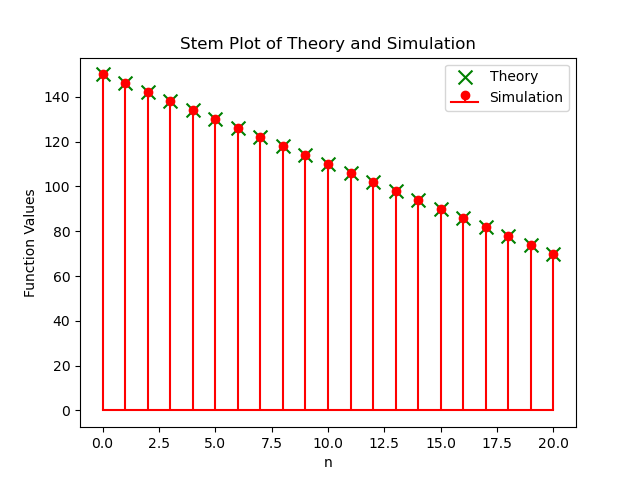
\includegraphics[width=1\linewidth]{Theory_vs_Simulation.png}
   \caption{Comparison of Theory and Simulated Values}
   \label{fig: 11.9.5.32.1}
 \end{figure}

\end{document}

\pagebreak

\item The Fibonacci sequence is defined by 1 = a$1$ = a$_2$ and a$_n$ = a${n-1}$ + a$_{n-2}$ , n $\textgreater$ 2\\
Find $\dfrac{a_{n + 1}}{a_n}$, for n = 1, 2, 3, 4, 5\\
\solution
\input{ncert-maths/11/9/1/14/11-9.1-14.tex}
\pagebreak

\item  A farmer buys a used tractor for Rs 12000. He pays Rs 6000 in cash and agrees to pay the balance in annual installments of Rs 500 plus 12 \% interest on the unpaid amount. How much will the tractor cost him?
\solution
\input{ncert-maths/11/9/5/27/11.9.5.27.tex}
\pagebreak

\item 1) Find the sum to n terms for the given series: $3\times8 + 6\times11 + 9\times14 + ...$
\solution
\pagebreak

\item The sum of the first $n$ terms of two arithmetic progressions (AP) is in the ratio $5n+4 : 9n+6$. Find the ratio of their 18th terms.\\
\solution
\pagebreak

\item How many terms of the AP : 9, 17, 25, . . . must be taken to give a sum of 636?
\solution
\input{ncert-maths/10/5/3/4/ASS2.tex}
\pagebreak
\item How many terms of the A.P. -6,$-\frac{11}{2}$, -5, ..... are needed to give the sum -25?\\
\solution
\input{ncert-maths/11/9/2/4/assignment1.tex}
\pagebreak

\item Find the sum to indicated number of terms in the geometric progression:\\
1, $– a$, $a^2$
, $-a^3$
, ... n terms (if $a \neq – 1$).\\
\solution
\pagebreak

\item Let S be the sum, P the product and R the sum of reciprocals of n terms in a G.P.
Prove that $P^2 R^n = S^n$.\\
\solution
\pagebreak
\item Find the sum to n terms to the series $3\brak 1^2+5\brak 2^2+7\brak 3^2+ \ldots$\\
\solution
\input{ncert-maths/11/9/4/3/mp2.tex}
\pagebreak
\item Find the sum to n terms of the sequence $8,88,888,8888$\ldots\\
\solution\\
\input{ncert-maths/11/9/3/18/problem2.tex}
\pagebreak

\item If the first and the  $n^{th}$  term of a G.P. are $a$ and $b$, respectively, and if $P$ is the product of $n$ terms , prove that $ P^2 = \brak{ab}^n $ \\
\solution
 \iffalse
\let\negmedspace\undefined
\let\negthickspace\undefined
\documentclass[journal,12pt,twocolumn]{IEEEtran}
\usepackage{amssymb}
\usepackage{cite}
\usepackage{amsmath,amssymb,amsfonts,amsthm}
\usepackage{algorithmic}
\usepackage{graphicx}
\usepackage{textcomp}
\usepackage{xcolor}
\usepackage{txfonts}
\usepackage{listings}
\usepackage{enumitem}
\usepackage{mathtools}
\usepackage{gensymb}
\usepackage{comment}
\usepackage[breaklinks=true]{hyperref}
\usepackage{tkz-euclide} 
\usepackage{listings}
\usepackage{gvv}                                        
\def\inputGnumericTable{}                                 
\usepackage[latin1]{inputenc}                                
\usepackage{color}                                            
\usepackage{array}                                            
\usepackage{longtable}                                       
\usepackage{calc}                                             
\usepackage{multirow}                                         
\usepackage{hhline}                                           
\usepackage{ifthen}                                           
\usepackage{lscape}
\usepackage{pgfplots}
\newtheorem{theorem}{Theorem}[section]
\newtheorem{problem}{Problem}
\newtheorem{proposition}{Proposition}[section]
\newtheorem{lemma}{Lemma}[section]
\newtheorem{corollary}[theorem]{Corollary}
\newtheorem{example}{Example}[section]
\newtheorem{definition}[problem]{Definition}
\newcommand{\BEQA}{\begin{eqnarray}}
\newcommand{\EEQA}{\end{eqnarray}}
\newcommand{\define}{\stackrel{\triangle}{=}}
\theoremstyle{remark}
\newtheorem{rem}{Remark}
\begin{document}

\bibliographystyle{IEEEtran}
\vspace{3cm}

\title{NCERT Discrete-11.9.4-5}
\author{EE22BTECH11004 - Allu Lohith}

\maketitle
\newpage
\bigskip


 Find the sum of n terms of this sequence:$$5^2+6^2+7^2...+20^2$$  
\solution
\fi
\begin{table}[h!]
\centering
\renewcommand{\arraystretch}{2}
\begin{tabular}{|c|p{4cm}|c|}
\hline 
\setlength{\tabcolsep}{1pt}
\textbf{Parameter}  &\textbf{Description} &\textbf{Formulae/Value} \\
\hline
n & Iteration number starting from zero till 15 & - \\
\hline
$x\brak n$ & General term of the sequence from $n=0$ to $n=15$ &$\brak{n+5}^2$  u\brak n\\
\hline
$x\brak 0$ & First term of the sequence & 5 \\
\hline
\end{tabular}

\vspace{0.5cm}
\caption{\normalsize Parameters}
\end{table}
The standard $z$ transforms,
\begin{align}
    u \brak n &\stackrel{z}{\longleftrightarrow} \frac{1}{1-z^{-1}}, \abs z >1\\
   n u\brak n &\stackrel{z}{\longleftrightarrow} \frac{z^{-1}}{\brak{1-z^{-1}}^2}, \abs z >1\\
   n^2 u\brak n &\stackrel{z}{\longleftrightarrow} \frac{z^{-1}\brak{1+z^{-1}}}{\brak{1-z^{-1}}^3}, \abs z >1
\end{align}
As 
\begin{align}
    x\brak n = \brak{n^2+10n+25}u\brak n
\end{align}
The $z$ transform of general term can be written as , 
\begin{align}
    X\brak z &= \frac{z^{-1}\brak{1+z^{-1}}}{\brak{1-z^{-1}}^3}+10\frac{z^{-1}}{\brak{1-z^{-1}}^2}+\frac{25}{1-z^{-1}} \\
    X\brak z &=  \frac{16z^{-2}-39z^{-1}+25}{\brak{1-z^{-1}}^3}; \abs{z}>1
\end{align}
On convolution for finding the sum
\begin{align}
    y\brak n= x\brak n \ast u\brak n
\end{align}
On z transform,
\begin{align}
    Y\brak z &= X \brak z \cdot U \brak z\\
    &= \brak{\frac{16z^{-2}-39z^{-1}+25}{\brak{1-z^{-1}})^3}} \cdot \frac{1}{1-z^{-1}}\\
    \implies 
    Y \brak z & = \frac{16z^{-2}-39z^{-1}+25}{\brak{1-z^{-1}}^4}; \quad \abs z >1
\end{align}
Using the contour integration to find the inverse $z$ transform,
\begin{align}
    y(n)&=\oint_c Y(z)\cdot z^{n-1}dz\\
    y(21)&=\oint_c \brak{\frac{16z^{-2}-39z^{-1}+25}{\brak{1-z^{-1}}^4}} z^{14}dz
\end{align}
As there are four poles from observation, so $m=4$
\begin{align}
    y\brak{21} &= \frac{1}{(m-1)!} \lim_{z \to a} \frac{d^{m-1}}{dz^{m-1}}\brak{(z-a)^mf(z)}\\
    &= \frac{1}{3!} \lim_{z \to 1} \frac{d^{3}}{dz^{3}}\brak{(z-1)^4 \frac{\brak{16z^{-2}-39z^{-1}+25}}{(1-z^{-1})^4} z^{14}}\\
    &= \frac{1}{6} \lim_{z \to 1} \frac{d^{3}}{dz^{3}}\brak{\brak{16z^{-2}-39z^{-1}+25}z^{18}}\\
    &= \frac{1}{6} \lim_{z \to 1} \frac{d^{3}}{dz^{3}}\brak{16z^{16}-39z^{17}+25z^{18}}\\
    &= \frac{1}{6}  \brak{16 \times 18 \times 17 \times 16+14 \times 17 \times 16 \times 15 }\\
    \implies y\brak{21}&=2840 
\end{align}
Hence the sum of the terms of the sequence is 2840.

\begin{figure}[h]
    \centering  

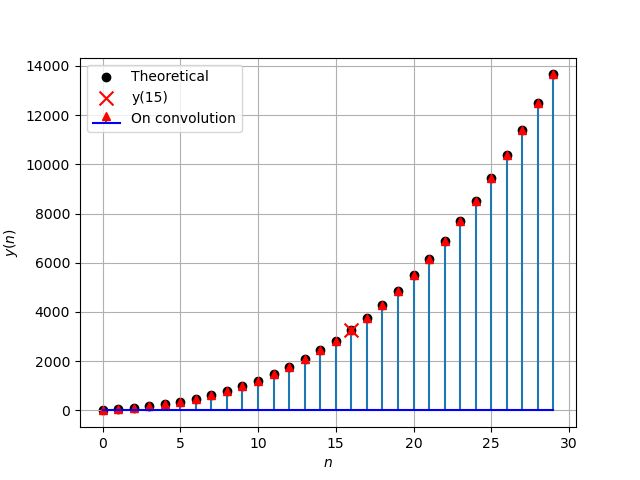
\includegraphics[width=\columnwidth]{ncert-maths/11/9/4/5/figs/plot.png}

\begin{center}
    \caption{Simulation v/s theoretical}
\end{center}
\end{figure}


\pagebreak

\item Between 1 and 31, m numbers have been inserted in such a way that the resulting sequence is an A.P. and 
the ratio of 7 th and (m - 1) th numbers is 5:9. Find the value of m.\\
\solution
\input{ncert-maths/11/9/2/16/1.tex}
\pagebreak
\item Find the sum of n terms of this sequence:$$5^2+6^2+7^2...+20^2$$  \\
\solution
 \iffalse
\let\negmedspace\undefined
\let\negthickspace\undefined
\documentclass[journal,12pt,twocolumn]{IEEEtran}
\usepackage{amssymb}
\usepackage{cite}
\usepackage{amsmath,amssymb,amsfonts,amsthm}
\usepackage{algorithmic}
\usepackage{graphicx}
\usepackage{textcomp}
\usepackage{xcolor}
\usepackage{txfonts}
\usepackage{listings}
\usepackage{enumitem}
\usepackage{mathtools}
\usepackage{gensymb}
\usepackage{comment}
\usepackage[breaklinks=true]{hyperref}
\usepackage{tkz-euclide} 
\usepackage{listings}
\usepackage{gvv}                                        
\def\inputGnumericTable{}                                 
\usepackage[latin1]{inputenc}                                
\usepackage{color}                                            
\usepackage{array}                                            
\usepackage{longtable}                                       
\usepackage{calc}                                             
\usepackage{multirow}                                         
\usepackage{hhline}                                           
\usepackage{ifthen}                                           
\usepackage{lscape}
\usepackage{pgfplots}
\newtheorem{theorem}{Theorem}[section]
\newtheorem{problem}{Problem}
\newtheorem{proposition}{Proposition}[section]
\newtheorem{lemma}{Lemma}[section]
\newtheorem{corollary}[theorem]{Corollary}
\newtheorem{example}{Example}[section]
\newtheorem{definition}[problem]{Definition}
\newcommand{\BEQA}{\begin{eqnarray}}
\newcommand{\EEQA}{\end{eqnarray}}
\newcommand{\define}{\stackrel{\triangle}{=}}
\theoremstyle{remark}
\newtheorem{rem}{Remark}
\begin{document}

\bibliographystyle{IEEEtran}
\vspace{3cm}

\title{NCERT Discrete-11.9.4-5}
\author{EE22BTECH11004 - Allu Lohith}

\maketitle
\newpage
\bigskip


 Find the sum of n terms of this sequence:$$5^2+6^2+7^2...+20^2$$  
\solution
\fi
\begin{table}[h!]
\centering
\renewcommand{\arraystretch}{2}
\begin{tabular}{|c|p{4cm}|c|}
\hline 
\setlength{\tabcolsep}{1pt}
\textbf{Parameter}  &\textbf{Description} &\textbf{Formulae/Value} \\
\hline
n & Iteration number starting from zero till 15 & - \\
\hline
$x\brak n$ & General term of the sequence from $n=0$ to $n=15$ &$\brak{n+5}^2$  u\brak n\\
\hline
$x\brak 0$ & First term of the sequence & 5 \\
\hline
\end{tabular}

\vspace{0.5cm}
\caption{\normalsize Parameters}
\end{table}
The standard $z$ transforms,
\begin{align}
    u \brak n &\stackrel{z}{\longleftrightarrow} \frac{1}{1-z^{-1}}, \abs z >1\\
   n u\brak n &\stackrel{z}{\longleftrightarrow} \frac{z^{-1}}{\brak{1-z^{-1}}^2}, \abs z >1\\
   n^2 u\brak n &\stackrel{z}{\longleftrightarrow} \frac{z^{-1}\brak{1+z^{-1}}}{\brak{1-z^{-1}}^3}, \abs z >1
\end{align}
As 
\begin{align}
    x\brak n = \brak{n^2+10n+25}u\brak n
\end{align}
The $z$ transform of general term can be written as , 
\begin{align}
    X\brak z &= \frac{z^{-1}\brak{1+z^{-1}}}{\brak{1-z^{-1}}^3}+10\frac{z^{-1}}{\brak{1-z^{-1}}^2}+\frac{25}{1-z^{-1}} \\
    X\brak z &=  \frac{16z^{-2}-39z^{-1}+25}{\brak{1-z^{-1}}^3}; \abs{z}>1
\end{align}
On convolution for finding the sum
\begin{align}
    y\brak n= x\brak n \ast u\brak n
\end{align}
On z transform,
\begin{align}
    Y\brak z &= X \brak z \cdot U \brak z\\
    &= \brak{\frac{16z^{-2}-39z^{-1}+25}{\brak{1-z^{-1}})^3}} \cdot \frac{1}{1-z^{-1}}\\
    \implies 
    Y \brak z & = \frac{16z^{-2}-39z^{-1}+25}{\brak{1-z^{-1}}^4}; \quad \abs z >1
\end{align}
Using the contour integration to find the inverse $z$ transform,
\begin{align}
    y(n)&=\oint_c Y(z)\cdot z^{n-1}dz\\
    y(21)&=\oint_c \brak{\frac{16z^{-2}-39z^{-1}+25}{\brak{1-z^{-1}}^4}} z^{14}dz
\end{align}
As there are four poles from observation, so $m=4$
\begin{align}
    y\brak{21} &= \frac{1}{(m-1)!} \lim_{z \to a} \frac{d^{m-1}}{dz^{m-1}}\brak{(z-a)^mf(z)}\\
    &= \frac{1}{3!} \lim_{z \to 1} \frac{d^{3}}{dz^{3}}\brak{(z-1)^4 \frac{\brak{16z^{-2}-39z^{-1}+25}}{(1-z^{-1})^4} z^{14}}\\
    &= \frac{1}{6} \lim_{z \to 1} \frac{d^{3}}{dz^{3}}\brak{\brak{16z^{-2}-39z^{-1}+25}z^{18}}\\
    &= \frac{1}{6} \lim_{z \to 1} \frac{d^{3}}{dz^{3}}\brak{16z^{16}-39z^{17}+25z^{18}}\\
    &= \frac{1}{6}  \brak{16 \times 18 \times 17 \times 16+14 \times 17 \times 16 \times 15 }\\
    \implies y\brak{21}&=2840 
\end{align}
Hence the sum of the terms of the sequence is 2840.

\begin{figure}[h]
    \centering  

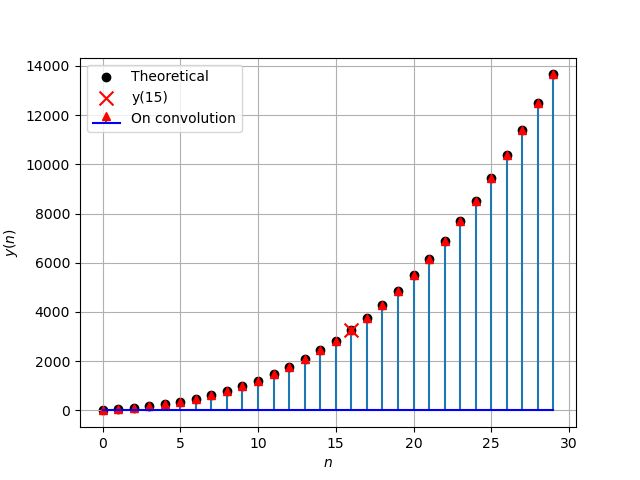
\includegraphics[width=\columnwidth]{ncert-maths/11/9/4/5/figs/plot.png}

\begin{center}
    \caption{Simulation v/s theoretical}
\end{center}
\end{figure}


\pagebreak

\item In an A.P., if the $p$-th term is $\frac{1}{q}$ and $q$-th term is $\frac{1}{p}$, prove that the sum of the first $pq$ terms is $\frac{1}{2}\brak{pq + 1}$, where $p \neq q$.\\
\solution
\input{ncert-maths/11/9/2/5/discrete.tex}
\pagebreak
\item Find the sum of n terms of the series:
$1\times2+2\times3+3\times4+4\times5+....$\\
\solution
\input{ncert-maths/11/9/4/1/Assignment11.9.4.1.tex}
\pagebreak

\end{enumerate}
